% ====================================================================
% graphite_ica_ch1_v8-11.tex — Chapter 1 (v8-11: 유도 확장판 9+9+1+1 최종본)
%   v8-10(체리픽) 을 adversarial 재검수(Phase6, 확정 CRIT/HIGH 0) 후 LOW 폴리시 보강한 최종.
%   보강: eq:Veq 출발 다리 가시화·fig:relaxode 캡션 정리(작가메모 제거)·eq:weff s-상쇄 명시·z_cut 선택값 명시.
%   불가침: 부호 8/8·11식 G-derive(SymPy/NumPy 검증)·D-PEAK/D-PEAK2·D-WEFF·결과 박스·코드 정합·그림 9.
%   ── 이하 v8-10(= v8-06b 베이스) 원형 ──
% graphite_ica_ch1_v8-10.tex — Chapter 1 (v8-10: 유도 확장판 9+9 경쟁·검토 체리픽 통합본)
%   베이스 = v8-06b(검토2 34/35·전 KNOWN_DEFECTS 해소·D-PEAK 2곳 정확·9 figs), v6 합류 교차검증.
%   보강 = D-PEAK2(eq:branch 문턱 진폭 불연속 = 이산 모드 스위치 정직 기술).
%   그림 경쟁 승자 = v7-11 유래 5 + 신규 4(검토2 청정). 이식금지 회귀: v8-02/03 D-PEAK 재정정·D-WEFF ¼·v8-07 s_F orphan.
%   ── 이하 베이스 v8-06b 원형 ──
% graphite_ica_ch1_v8-06.tex — Chapter 1 (v8-06: 유도 과정 포함 교과서 확장판)
%   배치·결과 박스·식별자·부호·표 = v7-11.tex 보존(절 순서 N0->N9·결과 박스 9식·
%   그림 5개·표 3종·부호 검산 절). v7 가 압축한 중간 유도를 v5 유도 원천에서
%   가져와 이 배치에 맞춰 다시 전개(베끼지 않음) — 각 결과 박스 위에
%   (a) 출발식/전제 -> (b) 적용 연산 -> (c) 중간식 >=1 -> (d) 박스 의 단계가 보인다.
%   유도 원천 = graphite_ica_ch1_Opus_v5.tex(통계역학 전 유도). 결과·부호 정본 =
%   Anode_Fit_v11_final.py(706줄). 무관 일반론(lever/chord·Marcus·KWW·적층·
%   master 알고리즘 S0-S5)은 결과 박스로 수렴하지 않으므로 재유입 안 함.
%   그림 = v7-11 의 5개(spine·staging·hysloop·logistic·reversal) 보존 + 유도를
%   돕는 신규 4개(activation barrier·flux crossing·double-well·relaxation ODE).
%   내부 텍스트 영어 ASCII 만.
%   build: xelatex -interaction=nonstopmode 2-pass (kotex — 한글 전제).
% ====================================================================
\documentclass[11pt,a4paper]{article}
\usepackage[margin=22mm]{geometry}
\usepackage{kotex}
\setmonofont{D2Coding}[Scale=MatchLowercase]
\usepackage{amsmath,amssymb,mathtools,bm}
\usepackage{booktabs,longtable,array}
\usepackage{enumitem}
\usepackage{amsthm}
\usepackage{hyperref}
\usepackage{fancyhdr}
\usepackage{lastpage}
\usepackage{setspace}
\usepackage{tikz}
\usetikzlibrary{positioning,arrows.meta,calc,fit,backgrounds}
\setstretch{1.12}
\setlength{\parskip}{0.45em}\setlength{\parindent}{0pt}\setlength{\headheight}{14pt}
\setlength{\emergencystretch}{2em}
\hypersetup{colorlinks=true, linkcolor=blue, urlcolor=blue, citecolor=blue,
  pdftitle={흑연 음극 + LCO 양극 dQ/dV 이론: 코드 진행을 따라가는 수식-구동 (유도 확장) — Chapter 1 (v9)}}
\pagestyle{fancy}\fancyhf{}
\lhead{흑연 음극 + LCO 양극 $dQ/dV$ 이론 — Ch.1 (v9, 코드 진행 + 유도)}\rhead{\thepage/\pageref{LastPage}}
\renewcommand{\headrulewidth}{0.4pt}

\newtheorem*{keybox}{핵심}
\newtheorem*{codebox}{코드 대응}
\newtheorem*{signbox}{부호 검산}
\newtheorem*{verifybox}{검산}
\newtheorem*{derivbox}{유도}

\newcommand{\dd}{\mathrm{d}}
\newcommand{\eff}{\mathrm{eff}}
\newcommand{\eq}{\mathrm{eq}}
\newcommand{\app}{\mathrm{app}}
\newcommand{\cell}{\mathrm{cell}}
\newcommand{\bg}{\mathrm{bg}}
\newcommand{\rxn}{\mathrm{rxn}}
\newcommand{\dis}{\mathrm{dis}}
\newcommand{\chg}{\mathrm{chg}}
\newcommand{\hys}{\mathrm{hys}}
\newcommand{\work}{\mathrm{work}}
\newcommand{\rep}{\mathrm{rep}}
\newcommand{\code}[1]{\texttt{#1}}

\renewcommand{\theequation}{1.\arabic{equation}}
\renewcommand{\thesection}{1.\arabic{section}}
\title{\textbf{\LARGE Chapter 1}\\[0.35em]\Large 흑연 음극 + LCO 양극 $dQ/dV$ 이론: 한 곡선을 그리는 코드 진행을 따라가는 수식-구동판 — 유도 확장}
\author{}
\date{}

\makeatletter
\renewcommand*\l@section[2]{%
  \ifnum \c@tocdepth >\z@
    \addpenalty\@secpenalty
    \addvspace{1.0em \@plus\p@}%
    \setlength\@tempdima{2.3em}%
    \begingroup
      \parindent \z@ \rightskip \@pnumwidth
      \parfillskip -\@pnumwidth
      \leavevmode \bfseries
      \advance\leftskip\@tempdima
      \hskip -\leftskip
      #1\nobreak\hfil
      \nobreak\hb@xt@\@pnumwidth{\hss #2\kern-\p@\kern\p@}\par
    \endgroup
  \fi}
\renewcommand*\l@subsection{\@dottedtocline{2}{2.3em}{3.2em}}
\makeatother

\begin{document}
\maketitle

% ====================================================================
\section*{서론 — 이 문건이 따라가는 것}
\addcontentsline{toc}{section}{서론}
% ====================================================================
리튬이온전지 흑연 음극의 incremental capacity analysis(ICA)는 충방전 곡선 $Q(V)$ 의 미분
$\dd Q/\dd V$ 를 본다 \cite{bloom2005,dubarry2012}. 흑연은 staging 상전이(stage
$4\!\to\!3\!\to\!2\mathrm L\!\to\!2\!\to\!1$)를 거치며 \cite{dahn1991,ohzuku1993}, 각 전이 전위에서
두 상이 공존하면 전위가 거의 평탄해 좁은 $\dd V$ 에 큰 $\dd Q$ 가 몰려 $\dd Q/\dd V$ 가 치솟는다.

본 문건은 이 곡선을 \emph{한 번 그리는 계산}을 그대로 따라간다. 계산은 구현 \code{Anode\_Fit\_v11\_final.py}
의 메서드 \code{dqdv} 한 번 호출이며, 그 내부는 아홉 단계 $\mathrm N0\!\to\!\mathrm N9$ 를 순서대로 밟는다
(그림~\ref{fig:spine}). 각 절은 그 한 단계에서 코드가 평가하는 물리식을, 그 단계를 이해하는 데 필요한 만큼
\emph{유도}한다 — 결과식만 나열하지 않고, 출발 전제에서 그 식까지 가는 중간 단계를 빠짐없이 보인다(이것이 v7
계열에서 압축됐던 부분이다). 곡선에 들어가지 않는 일반론은 결과식이 쓰이는 한에서만 최소로 인용한다. 도착점은 한 줄
합산식과, ``이 문건만 보고 같은 곡선을 재현하는 코드를 짤 수 있다''는 실행 가능성이다.

\textbf{관측.}
\begin{quote}\itshape
$\dd Q/\dd V$ 상전이 peak 의 위치$\cdot$너비$\cdot$높이는 (a) 온도 $T$, (b) 극판 전위, (c) C-rate(전류)
세 가지에 따라 변한다. 저온$\cdot$고율일수록 peak 의 꼬리가 길어져 다음 peak 와 겹치고, 같은 전이가 충전과 방전에서
서로 다른 전위에 peak 를 남기며(충방전 히스테리시스), 이 갈림에는 전류를 $0$ 으로 줄여도 사라지지 않는 성분이 있다.
\end{quote}

세 인자는 모두 하나의 속도식 $k\simeq k_0\exp[-\Delta G_a/RT]$ 의 서로 다른 자리로 들어온다 — 온도는 지수의 분모,
전위는 장벽 $\Delta G_a$ 자체, C-rate 는 요구 속도와 공급 속도의 경쟁이다. 이 속도식이 한편으로는 평형(정$\cdot$역
속도가 같아지는 정지점)을, 다른 한편으로는 유한 전류의 지연(꼬리)을 낳는다 — 본 문건의 유도는 줄곧 이 한 식의 가지를
펼치는 일이다. 코드 진행이 이 세 갈래를 차례로 닫는다.

\begin{figure}[t]
\centering
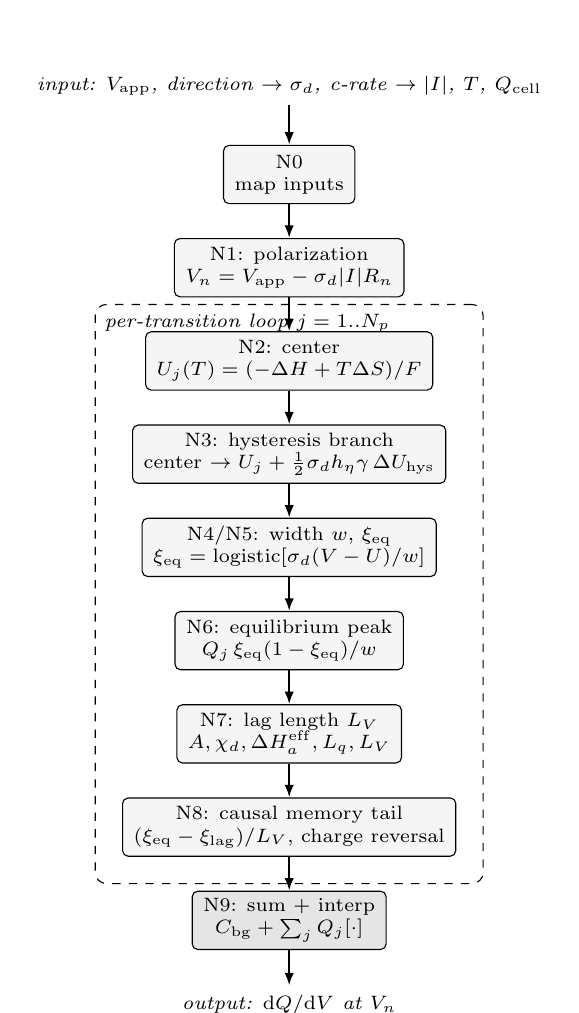
\begin{tikzpicture}[
  node distance=4.3mm and 5.5mm,
  stage/.style={draw,rounded corners=2pt,minimum height=7.4mm,inner xsep=4pt,inner ysep=2.5pt,font=\scriptsize,align=center,fill=black!4},
  core/.style={stage,fill=black!10},
  io/.style={font=\scriptsize\itshape,align=center},
  ar/.style={-{Latex[length=1.6mm]},thick}]
% input row
\node[io] (in) {input: $V_\app$, direction $\to\sigma_d$, c-rate $\to|I|$, $T$, $Q_\cell$};
% spine
\node[stage,below=5mm of in] (n0) {N0\\map inputs};
\node[stage,below=of n0] (n1) {N1: polarization\\$V_n=V_\app-\sigma_d|I|R_n$};
\node[stage,below=of n1] (n2) {N2: center\\$U_j(T)=(-\Delta H+T\Delta S)/F$};
\node[stage,below=of n2] (n3) {N3: hysteresis branch\\center $\to U_j+\tfrac12\sigma_d h_\eta\gamma\,\Delta U_\hys$};
\node[stage,below=of n3] (n4) {N4/N5: width $w$, $\xi_\eq$\\$\xi_\eq=\mathrm{logistic}[\sigma_d(V-U)/w]$};
\node[stage,below=of n4] (n6) {N6: equilibrium peak\\$Q_j\,\xi_\eq(1-\xi_\eq)/w$};
\node[stage,below=of n6] (n7) {N7: lag length $L_V$\\$A,\chi_d,\Delta H_a^\eff,L_q,L_V$};
\node[stage,below=of n7] (n8) {N8: causal memory tail\\$(\xi_\eq-\xi_\mathrm{lag})/L_V$, charge reversal};
\node[core,below=of n8] (n9) {N9: sum + interp\\$C_\bg+\sum_j Q_j[\cdot]$};
\node[io,below=4.5mm of n9] (out) {output: $\dd Q/\dd V$ at $V_n$};
\foreach \a/\b in {in/n0,n0/n1,n1/n2,n2/n3,n3/n4,n4/n6,n6/n7,n7/n8,n8/n9,n9/out}
  \draw[ar] (\a) -- (\b);
% per-transition loop bracket
\begin{scope}[on background layer]
\node[draw,dashed,rounded corners,fit=(n2)(n3)(n4)(n6)(n7)(n8),inner sep=3.4mm,label={[font=\scriptsize\itshape,anchor=north west]north west:per-transition loop $j=1..N_p$}] (loop) {};
\end{scope}
\end{tikzpicture}
\caption{한 곡선을 그리는 코드 진행(spine). 외부 실험조건이 \code{curve} facade 에서 $(\sigma_d,|I|,T,Q_\cell)$
로 환산($\mathrm N0$)되어 코어 \code{dqdv} 로 들어가고, 분극으로 내부 전위 $V_n$ 을 얻은 뒤($\mathrm N1$),
전이 $j$ 마다 평형 중심$\cdot$히스 분기$\cdot$폭$\cdot$평형 점유$\cdot$평형 peak$\cdot$지연 길이$\cdot$인과 꼬리를
계산해($\mathrm N2$--$\mathrm N8$) 합산$\cdot$역보간한다($\mathrm N9$). 본 문건의 절 번호가 이 노드 순서다.
점선 상자가 코드의 전이 루프(\code{for tr in transitions}). 그림 출처 — v7-11 의 spine 그림을 그대로 채택했다.}
\label{fig:spine}
\end{figure}

\tableofcontents
\newpage

% ====================================================================
\section{기호와 규약, 실험조건 매핑 (N0)}\label{sec:notation}
% ====================================================================
계산의 진입점은 facade \code{curve}$(V_\app,\text{direction},\text{c\_rate},Q_\cell,T)$ 이고, 그 첫 일은 실험조건을
코어 \code{dqdv} 의 모델 입력으로 환산하는 것이다 — 이것이 노드 $\mathrm N0$ 다. 방향 문자열은 방향 부호 $\sigma_d$ 로,
C-rate 는 전류 크기 $|I|$ 로 바뀐다:
\begin{equation}
\sigma_d=\begin{cases}+1 & \text{방전(discharge)}\\ -1 & \text{충전(charge)}\end{cases},
\qquad
|I|=\text{c\_rate}\cdot Q_\cell\quad(\text{또는 }I_\mathrm{abs}\text{ 직접 지정}).
\label{eq:n0map}
\end{equation}
방향 부호의 작용처는 셋 — 분극 부호($\mathrm N1$), 분기 중심 선택($\mathrm N3$), 꼬리 지지 방향($\mathrm N8$) — 이며,
평형 종 자체는 방향 불변이다(아래에서 식으로 회수). 본 장이 뽑는 양은 $\dd Q/\dd V$ 한 곡선이다.

\textbf{전이 인덱스.} $j=1,\dots,N_p$($N_p\approx3$--$4$). 전이 $j$ 의 진행률 $\xi_j$(방전 시 $0\to1$ 로 증가, 곧 탈리튬화 진행),
용량 가중 $Q_j$. 박스 결과식은 $j$ 첨자를 단다. 점유율과 진행률은 $\theta_j=1-\xi_j$ 로 묶이며(점유 $\theta$ 가 $1\to0$
줄어드는 것이 진행 $\xi$ 가 $0\to1$ 느는 것), 유도에서 둘은 부호 한 번 차이로 오간다.

\textbf{부호 규약(★최우선 결함 클래스).} 전위는 흑연 음극 반쪽전지 전위(vs Li/Li$^+$)다. 방향 부호 $\sigma_d=\pm1$
(방전 $+1$/충전 $-1$)이 코드의 \code{s} 인자이며, 평형 점유 $\xi_\eq=\mathrm{logistic}[\sigma_d(V-U)/w]$ 에서 방전
($\sigma_d=+1$)은 $V\!\uparrow\Rightarrow\xi_\eq\!\uparrow$(전위를 올리면 탈리튬화). 분기 중심 $\pm\tfrac12\sigma_d(\cdots)$
는 방전$\cdot$충전이 반대로 갈리고, 꼬리는 충전에서 격자 역전을 받는다. 이 규약은 \S\ref{sec:notation}--\S\ref{sec:sum}
전건에서 유지되며 \S\ref{sec:signcheck} 가 전수 검산한다.

\begin{longtable}{p{0.17\textwidth} p{0.16\textwidth} p{0.585\textwidth}}
\toprule 기호(코드 식별자) & 단위 & 의미 \\ \midrule \endhead
\multicolumn{3}{l}{\emph{— 실험조건$\cdot$방향(N0$\cdot$N1) —}}\\
$\sigma_d$ (\code{s},\,\code{sigma\_d}) & --- & 방향 부호 — 방전 $+1$/충전 $-1$ \\
$|I|$ (\code{I\_abs}) & A & 전류 크기 $=$ c\_rate$\cdot Q_\cell$ \\
$Q_\cell$ (\code{Q\_cell}) & C & 셀 용량(전하); $q=Q/Q_\cell$ 환산$\cdot$$|I|$ 환산 공용 \\
$T$ (\code{T}) & K & 온도 — 스칼라(등온) 또는 $V_\app$ 길이 배열($T(V)$ 비등온) \\
$R_n$ (\code{Rn}) & $\Omega$ & 음극 lumped 분극 저항 \\
$V_\app$ (\code{V\_app}) & V & 인가(측정) 전위 격자 \\
$V_n$ & V & 내부(열역학) 전위 $=V_\app-\sigma_d|I|R_n$ \\
\multicolumn{3}{l}{\emph{— 평형 중심$\cdot$폭$\cdot$점유(N2$\cdot$N4$\cdot$N5) —}}\\
$U_j(T)$ (\code{U},\,\code{func\_U\_j}) & V & 전이 $j$ 평형 중심 전위 $=(-\Delta H_\rxn+T\Delta S_\rxn)/F$ \\
$\Delta H_{\rxn,j},\Delta S_{\rxn,j}$ (\code{dH\_rxn},\code{dS\_rxn}) & {\footnotesize J/mol;\,J/(mol\,K)} & 삽입 \emph{반응} 엔탈피$\cdot$엔트로피(평형 — \emph{활성화}와 다름) \\
$n_j$ (\code{n}) & --- & 폭 다중도($w=n_jRT/F$; \code{w} 주면 $n=wF/RT$ 역산) \\
$w_j$ (\code{func\_w}/\code{func\_w\_eff}) & V & 전이 폭 척도 $=n_jRT/F$(옵션 $w^\eff$) \\
$\xi_{\eq,j}$ (\code{func\_ksi\_eq}) & --- & 평형 진행률(logistic) \\
$Q_j$ (\code{Q}) & C & 전이 $j$ 용량 가중 \\
$C_\bg$ (\code{Cbg}) & C/V & 배경 미분용량(상수 또는 $V$ 함수) \\
\multicolumn{3}{l}{\emph{— 히스테리시스 분기(N3) —}}\\
$\Omega_j$ (\code{Omega}) & J/mol & 정규용액 상호작용 에너지($>2RT$ 면 상분리$\cdot$히스) \\
$\gamma_j$ (\code{gamma}) & --- & 분기 축소 인자 $0\le\gamma_j\le1$($0$ 이면 분기 없음) \\
$\Delta U_j^\hys$ (\code{func\_dU\_hys}) & V & spinodal 상한 분기 gap \\
$h_{\eta,j}$ (\code{h\_eta}) & --- & 부분 cycle 인자(기본 $1$) \\
$U_j^{\,d}$ (\code{center},\,\code{func\_U\_branch}) & V & 방향별 분기 중심 \\
\multicolumn{3}{l}{\emph{— 동역학 꼬리(N7$\cdot$N8) —}}\\
$\chi$ (\code{chi},\,\code{x}) & --- & 전이상태 분율 위치(전달 계수); 방향별 $\chi_d$ \\
$\chi_d$ (\code{func\_chi\_d}) & --- & 방향별 전달 계수 — 방전 $\chi$/충전 $1-\chi$ \\
$\mathcal A$ (\code{A}) & J/mol & 꼬리 컷점 affinity $=\min(z_\mathrm{cut}n_jRT,\,A_\mathrm{cap}RT)$ \\
$\Delta H_{a,j},\Delta S_{a,j}$ (\code{dH\_a},\code{dS\_a}) & {\footnotesize J/mol;\,J/(mol\,K)} & \emph{활성화} 엔탈피$\cdot$엔트로피(속도) \\
$\Delta H_{a,j}^\eff$ (\code{func\_dH\_a\_eff}) & J/mol & 유효 장벽 $=\Delta H_a-\chi_d\Omega$ \\
$L_{q,j}$ (\code{func\_L\_q}) & --- & 용량축 지연 길이 \\
$L_{V,j}$ (\code{lag\_len\_V}) & V & 전압축 지연 길이 $=|\dd V/\dd q|_{q_a}L_{q,j}$ \\
$|\dd V/\dd q|_{q_a}$ (\code{dVdq\_qa}) & V & 컷점 OCV 기울기($L_q\to L_V$ 환산) \\
$z_\mathrm{cut}$ (\code{z\_cut}) & --- & 컷 affinity 의 $z=\mathcal A/(n_jRT)$(기본 $4.357$) \\
$A_\mathrm{cap}$ (\code{A\_cap\_RT}) & --- & 컷 affinity 상한 배수(기본 $4.0$) \\
$\xi_{\mathrm{lag},j}$ (\code{occ\_lagged}) & --- & 인과 저역통과된 진행률 \\
\multicolumn{3}{l}{\emph{— 상수 —}}\\
$R,F,k_B,h$ & {\footnotesize J/(mol\,K), C/mol, J/K, J\,s} & 기체상수, Faraday, Boltzmann, Planck \\
\bottomrule
\end{longtable}

흑연 staging 의 갤러리 채움을 그림~\ref{fig:staging} 에 둔다 — 각 stage 전이가 한 peak 를 남기고, 코드의 전이 리스트
\code{GRAPHITE\_STAGING\_LIT}(4건)이 이 네 전이의 초기값이다.

\begin{figure}[t]
\centering
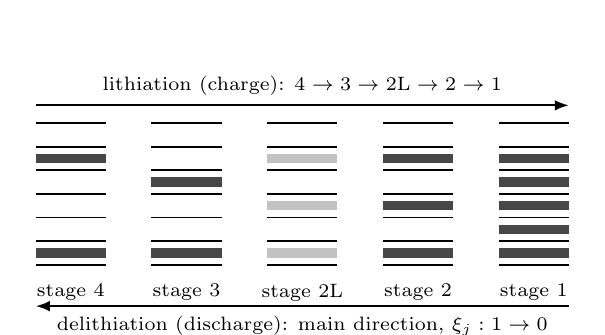
\begin{tikzpicture}[x=1.05cm,y=0.5cm,
  lab/.style={font=\scriptsize,align=center},
  fill4/.style={fill=black!72},fillL/.style={fill=black!24}]
% five stage columns, each shows graphene layers (lines) and Li-filled galleries (bands)
% column x-centers
\def\colw{0.85}
% stage 4: 1 filled gallery of 4
\foreach \x/\name/\filled/\style in {0/{stage 4}/{1}/fill4, 1.4/{stage 3}/{1}/fill4, 2.8/{stage 2L}/{all}/fillL, 4.2/{stage 2}/{all}/fill4, 5.6/{stage 1}/{dense}/fill4}{
  \draw[semithick] (\x,0)--(\x+\colw,0);
  \foreach \k in {1,2,3,4,5,6}{\draw[semithick] (\x,0.6*\k)--(\x+\colw,0.6*\k);}
  \node[lab,below] at (\x+\colw/2,-0.25) {\name};
}
% galleries (bands between layers) — explicit per column for clarity
% stage 4: every 4th gallery filled
\foreach \k in {1,5}{\fill[black!72] (0,0.6*\k-0.42) rectangle (0+\colw,0.6*\k-0.18);}
% stage 3: every 3rd
\foreach \k in {1,4}{\fill[black!72] (1.4,0.6*\k-0.42) rectangle (1.4+\colw,0.6*\k-0.18);}
% stage 2L: every 2nd, light (liquid-like)
\foreach \k in {1,3,5}{\fill[black!24] (2.8,0.6*\k-0.42) rectangle (2.8+\colw,0.6*\k-0.18);}
% stage 2: every 2nd, dark
\foreach \k in {1,3,5}{\fill[black!72] (4.2,0.6*\k-0.42) rectangle (4.2+\colw,0.6*\k-0.18);}
% stage 1: all galleries
\foreach \k in {1,2,3,4,5}{\fill[black!72] (5.6,0.6*\k-0.42) rectangle (5.6+\colw,0.6*\k-0.18);}
\draw[-{Latex[length=1.8mm]},thick] (0,4.05)--(6.45,4.05) node[pos=0.5,above,font=\scriptsize] {lithiation (charge): $4\to3\to2\mathrm L\to2\to1$};
\draw[{Latex[length=1.8mm]}-,thick] (0,-1.05)--(6.45,-1.05) node[pos=0.5,below,font=\scriptsize] {delithiation (discharge): main direction, $\xi_j:1\to0$};
\end{tikzpicture}
\caption{흑연 staging 의 갤러리 채움 도식(v7-11 유래, 그대로 채택). 수평선이 그래핀 층, 음영 띠가 리튬이 든 층간 갤러리다.
채울수록 stage 번호가 줄어 stage 1($\mathrm{LiC_6}$, 완전 채움)에 닿고, 각 stage 전이가 $\dd Q/\dd V$ 에 peak
하나를 남긴다. stage $2\mathrm L$ 은 면내 질서가 풀린 단계라 옅게 표시했다. 코드의 전이 리스트 4건이 이 전이들의
초기값이며($U\approx0.21/0.14/0.12/0.085$ V), 본 문건 방향은 방전(탈리튬화)이다.}
\label{fig:staging}
\end{figure}

\subsection{두 번째 전극 — LCO 양극으로의 일반화}\label{sec:lco-map}
지금까지의 기호와 매핑은 \emph{전극을 가리지 않는다} — 식~\eqref{eq:n0map} 의 방향 부호$\cdot$전류 환산, 전이 인덱스
$j$, 진행률 $\xi_j$, 평형 중심 $U_j$ 는 삽입형 전극이면 어디서나 같은 골격이다. 이 절은 같은 골격을 두 번째 사례인
$\mathrm{LiCoO_2}$(LCO) 양극에 \emph{건다}. 흑연 서술은 한 줄도 바뀌지 않으며(아래 모든 흑연 식$\cdot$표$\cdot$부호는
불변), LCO 는 ``파라미터를 갈아 끼우고 고유 항 하나를 더하는'' 두 번째 전극으로 들어온다. 본 문건이 다루는 범위는
\emph{코인 하프셀}(LCO vs Li metal) 단독이다 — 전셀 합성($\partial U_\cell=\partial U_\mathrm{cat}-\partial U_\mathrm{an}$)은
범위 밖이며(후속), 단전극 부호와 전셀 부호를 섞지 않는다.

\textbf{양극 부호 규약(흑연과 1:1 대칭).} LCO 하프셀 전위는 vs Li/Li$^+$ 로 $\sim$3.9--4.2 V 영역에 있다 — 흑연 음극의
$\sim$0.1 V 와 달리 \emph{높은} 전위다. 그러나 부호 골격은 같다: 방전($\sigma_d=+1$)은 LCO 입장에서 \emph{리튬화}
(Li$^+$ 가 LCO 로 들어와 Co$^{4+}\!\to$Co$^{3+}$ 환원, $x$ 증가, 전위 하강)이고, 충전($\sigma_d=-1$)은 \emph{탈리튬화}
($x$ 감소, 전위 상승)이다. 평형 중심의 온도 의존 $\partial U_j/\partial T=\Delta S_{\rxn,j}/F$(식~\eqref{eq:Uj} 미분)는
부호까지 흑연과 동일한 관계식이며, 부호의 \emph{값}만 전이별 $\Delta S_{\rxn,j}^\mathrm{cat}$ 가 정한다(\S\ref{sec:lco-center}).
흑연에서 $\xi_j$ 가 탈리튬화 진행이었듯, LCO 양극에서 충전(탈리튬화)이 $\xi:0\!\to\!1$ 의 주 진행 방향이다 — 본 문건의
LCO 전이표는 그 충전(탈리튬화) 진행을 전위 오름차순으로 적는다.

흑연의 \code{GRAPHITE\_STAGING\_LIT}(표~\ref{tab:staging})에 대응하는 LCO 초기값 리스트를
\code{LCO\_STAGING\_LIT} 로 둔다 — 표~\ref{tab:lco-staging} 가 그 세 전이다. 흑연이 4 staging 전이를 남기듯, LCO
하프셀(코인, $\le$4.2--4.5 V)은 세 전이를 남긴다\cite{xia2007}: $\sim$3.90 V 의 절연체$\to$금속 천이(MIT), $\sim$4.05 V 와
$\sim$4.17 V 의 한 쌍 order--disorder 전이다(고전압 $\sim$4.55 V 의 O3$\to$H1-3 는 하프셀 상한이 $\le$4.2--4.5 V 면
범위 밖이라 옵션으로 둔다). 이 값들은 흑연과 마찬가지로 \emph{신뢰값이 아니라 초기값}이며(tier — 1차 문헌
Xia\cite{xia2007}$\cdot$Reynier\cite{reynier2004}$\cdot$Motohashi\cite{motohashi2009} 에서 읽은 출발점), 우리 시료 데이터로
피팅해 override 하는 전제다.

\begin{table}[t]
\centering\footnotesize
\renewcommand{\arraystretch}{1.3}
\caption{LCO 하프셀 전이 초기값 \code{LCO\_STAGING\_LIT}(3건, vs Li metal) — 출발점, 피팅으로 override. $x$ 는
$\mathrm{Li}_x\mathrm{CoO_2}$ 의 리튬 함량. ``성격''은 상전이 유형, ``전자항''은 \S\ref{sec:lco-electronic} 의 MIT
게이트 발현 여부. 흑연 표~\ref{tab:staging} 와 같은 자리(전위$\cdot$성격$\cdot\Delta S$), 양극 부호.}
\label{tab:lco-staging}
\begin{tabular}{@{}p{0.155\textwidth} c p{0.085\textwidth} p{0.165\textwidth} p{0.255\textwidth} p{0.115\textwidth}@{}}
\toprule
전이 & $U_j$ [V] & $x$ 범위 & 성격 & $\Delta S_{\rxn,j}^\mathrm{cat}$ 초기값 & 전자항 \\
\midrule
T1 (MIT)              & $\sim$3.90        & 0.94--0.75 & insulator$\to$metal       & config $+\,\Delta S_e$ 게이트 ON & \textbf{발현(핵심)} \\
T2 (order--disorder a)& $\sim$4.05        & $\approx$0.55 & hex$\to$monoclinic 정렬 & config 주도($\approx$0.47 J/K\,mol) & off \\
T3 (order--disorder b)& $\sim$4.17--4.20  & $\approx$0.48 & monoclinic$\to$hex      & config($\approx$1.49 J/K\,mol) & off \\
\midrule
(T4)                  & $\sim$4.55        & $\approx$0.2 & O3$\to$H1-3              & --- & (고전압, 범위 밖) \\
\bottomrule
\end{tabular}
\end{table}

흑연이 \code{GRAPHITE\_STAGING\_LIT} 의 $(\Delta H_\rxn,\Delta S_\rxn,Q,\Omega,\Delta H_a,\dots)$ 키를 전이별로 갖듯,
LCO 전이도 같은 키 구조를 갖되 값만 표~\ref{tab:lco-staging} 의 양극 영역으로 바뀐다. 단 하나의 구조적 차이는 T1 에
흑연엔 없는 \emph{전자 엔트로피 항} $\Delta S_e(x,T)$ 가 더해지는 것이며(MIT 고유), 이것이 \S\ref{sec:lco-electronic}
의 새 절이다. 그 전까지(N1--N5)는 흑연과 LCO 가 \emph{같은 식}을 공유하므로, 다음 절들은 흑연으로 식을 세운 뒤 LCO
파라미터를 끼우는 순서로 간다.

% ====================================================================
\section{분극 — 측정 전위에서 내부 전위로 (N1)}\label{sec:pol}
% ====================================================================
코어 \code{dqdv} 의 첫 식은 분극을 벗기는 환산이다. 관측은 유한 전류에서 이루어지므로 측정 전위 $V_\app$ 에는 셀의
직렬 저항을 통과한 IR 분극이 실려 있고, 평형 열역학이 사는 전위는 그 분극을 벗긴 내부 전위 $V_n$ 이다.

\subsection{분극 부호 — 방향이 결정한다}
\textbf{(a) 출발 — 측정 전위와 내부 전위의 차.} 전류 크기 $|I|$ 가 lumped 저항 $R_n$ 을 통과하며 만드는 전위 강하는
크기 $|I|R_n$ 이고, 그 부호는 전류 방향이 정한다. 측정 전위는 내부 전위에 분극이 더해진 값이므로 한 방향(방전)에서
\begin{equation}
V_\app\;=\;V_n+\sigma_d\,|I|\,R_n
\qquad(\sigma_d=+1\ \text{방전})
\label{eq:vapppol}
\end{equation}
로 적는다 — 방전($\sigma_d=+1$)은 음극에서 산화(탈리튬화)가 일어나는 방향이라 측정 전위가 내부 전위보다 분극만큼
\emph{높게} 관측된다($V_\app>V_n$). 충전($\sigma_d=-1$)은 부호가 반대다. \textbf{(b) 연산 — $V_n$ 으로 이항.}
식~\eqref{eq:vapppol} 을 $V_n$ 에 대해 풀면(분극 항을 좌변으로 옮겨)
\begin{equation}
V_n\;=\;V_\app-\sigma_d\,|I|\,R_n,
\label{eq:vnmid}
\end{equation}
\textbf{(c) 두 방향을 한 식으로.} $\sigma_d$ 가 두 방향을 모두 흡수하므로 식~\eqref{eq:vnmid} 가 곧 박스다:
\begin{equation}
\boxed{\;V_n\;=\;V_\app\;-\;\sigma_d\,|I|\,R_n\;.}
\label{eq:vn}
\end{equation}
이것이 코드의 \code{V\_n = V\_in - sigma\_d * I\_abs * self.Rn} 한 줄이다. 부호 약속을 식으로 확인하면 —
방전에서 $V_n=V_\app-|I|R_n<V_\app$(측정이 내부보다 높음), 충전에서 $V_n=V_\app+|I|R_n>V_\app$ — 이며,
$|I|\to0$ 또는 $R_n=0$ 에서 $V_n=V_\app$ 로 두 전위가 일치한다.

\subsection{작업 격자 — 꼬리가 들어올 여유}
이후 모든 전이 계산은 $V_n$ 을 직접 쓰지 않고, $V_n$ 의 범위를 양쪽으로 넓힌 균일 \emph{작업 격자} $V_\work$ 위에서
이루어진다. 넓힘은 동역학 꼬리(\S\ref{sec:tail})가 격자 밖에서 잘려 인공 절단이 생기지 않도록 하는 여유다.
$v_\mathrm{lo}=\min V_n$, $v_\mathrm{hi}=\max V_n$, $\Delta v=v_\mathrm{hi}-v_\mathrm{lo}$ 로
\begin{equation}
V_\work=\mathrm{linspace}\big(v_\mathrm{lo}-p_\mathrm{lo}\,\Delta v,\;
v_\mathrm{hi}+p_\mathrm{hi}\,\Delta v,\;n_\work\big),
\qquad \Delta_\mathrm{grid}=V_{\work,1}-V_{\work,0},
\label{eq:vwork}
\end{equation}
패딩 $p_\mathrm{lo}=p_\mathrm{hi}=0.15$, 점 수 $n_\work=\max(2048,\,2\,|V_n|)$ 이다(코드 \code{grid\_pad\_lo/hi},
\code{n\_work\_min}). 온도가 배열 $T(V)$ 이면 같은 격자 위로 보간해 $T_\work$ 를 얻고($T_\mathrm{rep}=\overline{T_\work}$ 는
전이당 상수 평가용 대표 온도), 스칼라면 $T_\work\equiv T$ 다. 배경은 작업 격자 위에서 먼저 깔린다:
$\dd Q/\dd V|_\work \leftarrow C_\bg(V_\work)$. 모든 전이 기여는 여기에 더해지고($\mathrm N9$), 마지막에 $V_n$ 으로
역보간된다.

\begin{keybox}
\textbf{세 전위.} $V_\app$(측정)$\cdot$$V_n$(내부, 식~\eqref{eq:vn})$\cdot$$V_\work$(계산 격자, 식~\eqref{eq:vwork})는
지위가 다르다. 다음 절부터 평형$\cdot$동역학은 $V_\work$ 위에서 풀고, 출력만 $V_n$ 으로 되돌린다.
\end{keybox}

다음 절은 전이 루프의 첫 식 — 평형 중심 $U_j(T)$ — 으로 들어간다. 그 식이 어디서 오는지를 보이려면 먼저 평형을
판정하는 자유에너지 언어가 필요하므로, 다음 절은 $G\to\mu\to$ 평형 조건의 다리부터 놓는다.

% ====================================================================
\section{평형 중심 $U_j(T)$ — 열역학에서 (N2)}\label{sec:center}
% ====================================================================
전이 루프 안의 첫 물리량은 전이 $j$ 의 평형 중심 전위 $U_j(T)$ 다. 코드는 이를 열역학 입력 $(\Delta H_\rxn,\Delta S_\rxn)$
에서 \code{func\_U\_j} 로 계산하거나(없으면) \code{'U'} 를 직접 읽는다. 이 절은 그 환산식이 어디서 오는지를, Gibbs
자유에너지의 정의에서 한 단계씩 닫는다.

\subsection{$G,\mu$ 와 평형 조건 — 유도}
\textbf{(a) 출발 — 두 정의.} 등온$\cdot$등압 계(전지)의 자발성$\cdot$평형을 판정하는 퍼텐셜은 Gibbs 자유에너지
\begin{equation}
G\;\equiv\;H-TS
\label{eq:gibbsdef}
\end{equation}
이고($H$ 항과 $-TS$ 항이 경쟁하며 온도가 그 환율을 정한다), 입자 1몰 변화당 $G$ 변화가 화학퍼텐셜이다:
\begin{equation}
\mu\;\equiv\;\frac{\partial G}{\partial n}\Big|_{T,P}.
\label{eq:mudef}
\end{equation}
두 장소의 $\mu$ 일치가 입자 교환 평형이다. \textbf{(b) 연산 — 삽입 반응의 전기화학 평형.} 리튬은 Li$^+$ 와 $e^-$ 로
갈라져 드나들므로 각 종의 값어치에 전기 일 $zF\phi$(1몰)가 더해진 전기화학 퍼텐셜 $\tilde\mu\equiv\mu+zF\phi$ 가 균형을
이룬다. 삽입 반응 $\mathrm{Li}^++e^-+[\,]\rightleftharpoons\mathrm{Li}_{(\text{흑연})}$ 의 평형 조건
$\delta G=[\tilde\mu_\mathrm{Li}-\tilde\mu_{\mathrm{Li}^+}-\tilde\mu_{e^-}]\,\dd n=0$, 곧
\begin{equation}
\tilde\mu_{\mathrm{Li}^+}+\tilde\mu_{e^-}=\tilde\mu_\mathrm{Li}
\label{eq:eqbalance}
\end{equation}
에서, 전자 항이 $z=-1$ 이라 측정 전위 $V$ 를 통해 $\tilde\mu_{e^-}=\mu_{e^-}^0-FV$ 로 들어온다. \textbf{(c) 중간식 —
상수 덩이를 중심으로 흡수.} 좌변에서 $-FV$ 만 전위 의존이고 나머지(Li$^+$ 활동도$\cdot$기준 퍼텐셜)는 주어진 $T$ 에서
상수이므로, 그 상수 덩이를 $sFU$ 로 정의해($s=+1$ 라 $-FV=-sFV$) 묶으면 평형 조건이
\begin{equation}
\mu_\mathrm{Li}(\theta_\eq)\;=\;\mu^0-sF\,(V-U),
\qquad \Delta G_j\;=\;-sF\,U_j
\label{eq:eqcond}
\end{equation}
형태가 된다($s$ 는 방전 규약 $+1$; $U$ 는 비배치 몫 자유에너지의 전위 환산). \textbf{(d) 부호 핵심.} $\Delta G_j=-sFU_j$ —
$U_j$ 가 양이면 $\Delta G_j<0$, 곧 전이가 자발 진행할 전위가 양의 중심이다. 또한 $V$ 상승(전자 값어치 하락)$\Rightarrow$
평형 점유율 하강, 곧 ``$V$ 를 올리면 탈리튬화''가 이 한 식에 이미 들어 있다(\S\ref{sec:width} 의 logistic 부호로 회수).

\subsection{$U_j(T)$ — 온도 환산}
\textbf{(a) 출발.} 평형 조건의 비배치 몫은 반응 자유에너지 $\Delta G_j=\Delta H_{\rxn,j}-T\Delta S_{\rxn,j}$ 다.
\textbf{(b) 연산 — 식~\eqref{eq:eqcond} 의 $\Delta G_j=-sFU_j$($s=+1$)에 대입.} \textbf{(c) 중간식 — $U_j$ 로 이항.}
\begin{equation}
\Delta H_{\rxn,j}-T\Delta S_{\rxn,j}=-F\,U_j
\quad\Longrightarrow\quad
U_j=-\frac{\Delta H_{\rxn,j}-T\Delta S_{\rxn,j}}{F}
\label{eq:Ujmid}
\end{equation}
\textbf{(d) 박스 — 분자 부호 정리.}
\begin{equation}
\boxed{\;U_j(T)\;=\;\frac{-\Delta H_{\rxn,j}+T\,\Delta S_{\rxn,j}}{F}\;.}
\label{eq:Uj}
\end{equation}
이것이 \code{func\_U\_j(T, dH\_rxn, dS\_rxn)} 의 \code{(-dH\_rxn + T*dS\_rxn)/F} 다. 부호 — 발열 반응
$\Delta H_\rxn<0$ 이면 분자 $-\Delta H_\rxn>0$ 이 중심을 \emph{올린다}(흡열 아님에 주의). 온도 의존은 식~\eqref{eq:Uj} 를
$T$ 로 미분한 $\partial U_j/\partial T=\Delta S_{\rxn,j}/F$ 이고(Gibbs 항등식 $\partial\Delta G/\partial T=-\Delta S$ 와
식~\eqref{eq:eqcond} 의 $\Delta G=-FU$ 를 잇는 것과 같다), $|\Delta S_\rxn|\sim$ 수$\sim$수십 J/(mol\,K) 라 $30$ K
창에서 수 mV 규모로 중심이 이동한다 — 다온도 피팅에서 온도마다 $U_j(T)$ 를 따로 읽어야 하는 이유다. 코드가 배열
$T_\work$ 를 그대로 넣으므로 $U_j$ 는 비등온이면 격자별 배열로 나온다.

\begin{codebox}
\textbf{N2.} \code{if 'dH\_rxn' in tr and 'dS\_rxn' in tr: U\_j = func\_U\_j(T\_work, dH\_rxn, dS\_rxn)}
— 배열 $T_\work$ 대응. 없으면 \code{U\_j = float(tr['U'])} 직접. \code{GRAPHITE\_STAGING\_LIT} 의 stage 2$\to$1 은
$\Delta H_\rxn=-13000$ J/mol, $\Delta S_\rxn=-16$ J/(mol\,K) $\Rightarrow$ $U(298)=(13000-298.15\times16)/96485
\approx0.0853$ V(목표 $0.085$ V 정합).
\end{codebox}

\subsection{LCO 평형 중심과 $\partial U_j/\partial T$ — 양극 부호}\label{sec:lco-center}
식~\eqref{eq:Uj} 의 $U_j(T)=(-\Delta H_{\rxn,j}+T\Delta S_{\rxn,j})/F$ 는 \emph{유도에 전극 가정이 없다} — 평형 조건
식~\eqref{eq:eqcond}($\Delta G_j=-FU_j$)에서 곧장 나오므로 LCO 양극에도 그대로 성립한다. LCO 에 적용할 때 바뀌는 것은
입력 $(\Delta H_{\rxn,j},\Delta S_{\rxn,j})$ 의 \emph{값}뿐이고, 식과 부호 관계는 흑연과 1:1 이다. 양극 영역의 높은
중심($\sim$3.9--4.2 V)은 LCO 삽입 반응의 큰 음의 $\Delta H_\rxn$(분자 $-\Delta H_\rxn$ 가 크게 양)에서 온다 — 흑연의
$\sim$0.1 V 와 같은 식, 다른 입력.

온도 의존도 같은 미분이다:
\begin{equation}
\frac{\partial U_j}{\partial T}=\frac{\Delta S_{\rxn,j}^\mathrm{cat}}{F}
\qquad(\text{식~\eqref{eq:Uj} 의 }T\text{ 미분, 전극 불문}).
\label{eq:lco-dUdT}
\end{equation}
LCO 의 $\Delta S_{\rxn,j}^\mathrm{cat}$ 는 \S\ref{sec:lco-decomp} 에서 config$\cdot$vib$\cdot$전자 세 성분으로
분해되며, 여기서는 부호$\cdot$크기 sanity 만 확인한다 — LCO 단일전극(coin half-cell, vs Li) 엔트로피 계수의 \emph{대표
스케일}은 $\dd\phi/\dd T\approx+0.83$ mV/K 급이고(곧 $\Delta S_\rxn\approx+0.83\,\mathrm{mV/K}\times F\approx+80$
J/(mol\,K) 규모[tier B], 단 부호$\cdot$크기는 $x$ 의존이라 전이별 정밀값 아님). 이는 흑연의 $\Delta S_\rxn$(전이별
$+29/0/-5/-16$ J/(mol\,K), 표~\ref{tab:staging})과 \emph{값은 다르나}, 식~\eqref{eq:lco-dUdT} 의 관계
$\partial U_j/\partial T=\Delta S_{\rxn,j}/F$ 는 두 전극에서 동일한 형태로 성립한다.

\begin{verifybox}
\textbf{LCO 중심 부호 검산($T=298.15$ K).} 대표 단전극 엔트로피 계수 $\dd\phi/\dd T\approx+0.83$ mV/K\cite{swiderska2019}
(tier B — LCO \emph{단일전극} potentiometric, 크기$\cdot$부호 스케일 검증용 초기값)를 식~\eqref{eq:lco-dUdT}
에 역대입하면 $\Delta S_{\rxn}^\mathrm{cat}=F\,\dd U/\dd T=96485\times0.83\times10^{-3}\approx+80$ J/(mol\,K)$>0$ —
이 스케일에서 평형 중심이 온도에 \emph{오른다}($\partial U/\partial T>0$), $30$ K 창에서 $\Delta U\approx+25$ mV 규모다.
\textbf{★단전극 대 전셀 혼동 금지.} 이 $+0.83$ mV/K 는 \emph{LCO 단일전극}(vs Li, 본 문건 범위) 값이다 — 같은 문헌의
\emph{전셀}(LCO$-$graphite) 엔트로피 계수는 SOC 에 따라 부호가 전환되며($-0.37$\,\textasciitilde$+0.1$ mV/K) 흑연 항이
합산된 다른 양이다. 본 문건은 하프셀 범위라 단전극 LCO 부호만 쓴다(전셀 합성은 후속). 또한 $\dd\phi/\dd T$ 의 부호$\cdot$
크기는 $x$(SOC)에 의존하므로 위 $+0.83$ 은 \emph{대표 스케일}일 뿐 전이별 정밀값이 아니다 — 전이별 $\Delta S_{\rxn,j}^\mathrm{cat}$
는 표~\ref{tab:lco-staging}$\cdot$식~\eqref{eq:lco-decomp} 의 초기값을 데이터로 피팅해 정한다(허위 정밀 금지, tier 병기).
다온도 LCO 피팅에서 온도마다 $U_j(T)$ 를 따로 읽어야 함은 흑연보다 더 분명하다.
\textbf{★전자항과의 부호 공존(오독 방지).} 이 $\Delta S_{\rxn}^\mathrm{cat}\!\approx\!+80$ J/(mol\,K)$>0$ 은
단전극 전체 엔트로피 계수(config$+$vib$+$elec 세 성분의 \emph{합}, 식~\eqref{eq:lco-decomp})의 \emph{대표 스케일}이며,
T1 의 전자항 $\Delta S_{e,j}<0$(삽입 기준, \S\ref{sec:lco-electronic})과 모순되지 않는다 — 전자항은 몰당
$|\Delta S_e|\!\approx\!0.18\,k_B$/atom $\times N_A\!\approx\!1.5$ J/(mol\,K) 규모의 \emph{소수 음의 보정}이라, 그보다
훨씬 큰 양의 전체 합($\approx\!+80$)에 얹혀도 \emph{총 부호는 불변}($\approx\!+80>0$)이다. 한 가지 종류 혼동만
경계하면 된다 — 표~\ref{tab:lco-staging} 의 config$\cdot$vib 값은 \emph{전이별 부분몰} 성분이고 $+80$ 은 \emph{전체 계수}의
대표 스케일이라, 둘은 \emph{서로 다른 종류의 양}이다(\S\ref{sec:lco-decomp}). 곧 ``전체 계수의 $+80$''과
``T1 전자항 음수''(한 성분)는 모순이 아니라 서로 다른 층위에서 공존한다.
\end{verifybox}

다음은 같은 루프 안에서 이 중심을 충$\cdot$방전으로 갈라놓는 히스테리시스 분기다 — 그 갈림은 식~\eqref{eq:mudef} 의
$\mu$ 에 상호작용 몫이 들어가 평형이 비틀리는 데서 온다.

% ====================================================================
\section{히스테리시스 분기 중심 (N3)}\label{sec:hys}
% ====================================================================
코드는 평형 중심 $U_j$ 를 곧바로 쓰지 않고, 상호작용 $\Omega_j$ 와 분기 인자 $\gamma_j$ 가 있으면 방향별 분기 중심
$U_j^{\,d}$ 로 옮긴다. 본 문건의 주 전개는 방전이며, 히스테리시스는 그 위의 \emph{구조적 분기}로 선언된다 — 방전과 충전이
같은 전이를 서로 다른 준안정 가지로 과주행해 중심이 갈라진다(삽입형 전극 히스테리시스의 열역학적 기원\cite{dreyer2010}).
이 절은 그 gap 의 닫힌 식과 부호를, 격자기체 자유에너지의
이중웰에서 spinodal 을 거쳐 단계적으로 유도한다.

\subsection{상호작용이 평형을 비트는 곳 — $\mu(\theta)$ 의 상호작용 몫}
\textbf{(a) 출발 — 격자기체 $\mu$.} 한 전이를 ``동등한 자리에 리튬이 차고 비는'' 격자기체로 보면, 점유율 $\theta$ 의 화학
퍼텐셜은 섞임 엔트로피의 로그 몫과 정규용액 상호작용 몫의 합이다. 섞임 몫은 $N$ 자리에서 $n=N\theta$ 를 고르는 경우의
수 $W=N!/[n!(N-n)!]$ 에 Stirling 근사 $\ln m!\simeq m\ln m-m$ 을 적용해
$S_\mathrm{mix}=-k_BN[\theta\ln\theta+(1-\theta)\ln(1-\theta)]$ 로 닫히고, 상호작용 몫은 점유 이웃 쌍의 평균장 초과
에너지 $c\,\theta^2=c\theta+\Omega\theta(1-\theta)$($\Omega\equiv-c$, 선형 몫은 기준에 흡수)에서 온다. 자리 1몰당
자유에너지 $\bar g(\theta)=\mu^0\theta+RT[\theta\ln\theta+(1-\theta)\ln(1-\theta)]+\Omega\theta(1-\theta)$ 를
$\theta$ 로 미분하면(로그 몫은 $RT\ln[\theta/(1-\theta)]$, 상호작용 몫은 $\Omega(1-2\theta)$ — 상수 $\pm1$ 상쇄)
\begin{equation}
\mu_\mathrm{Li}(\theta)=\mu^0+RT\ln\frac{\theta}{1-\theta}+\Omega_j\,(1-2\theta).
\label{eq:mu}
\end{equation}
\textbf{(b) 연산 — 진행률 $\xi=1-\theta$ 로.} 자유에너지를 진행률 $\xi=1-\theta$ 로 옮기면, 1차(직선) 몫과 상수는
공통 접선 판정에 불변이라 떼어내고($g_j^0$ 으로 묶어) 조성 의존만 남긴다:
\begin{equation}
g_j(\xi)=g_j^0+RT\big[\xi\ln\xi+(1-\xi)\ln(1-\xi)\big]+\Omega_j\,\xi(1-\xi),
\label{eq:gxi}
\end{equation}
($\Omega>0$ 이면 동종 이웃 인력 — 가운데를 위로 밀어 이중웰의 씨앗). \textbf{(c) 중간식 — 두 번 미분.}
식~\eqref{eq:gxi} 를 두 번 $\xi$ 로 미분하면(로그 몫의 1계 미분 $RT\ln[\xi/(1-\xi)]$, 2계 미분
$RT/[\xi(1-\xi)]$; 상호작용 몫의 2계 미분 $-2\Omega$)
\begin{equation}
g_j''(\xi)=\frac{RT}{\xi(1-\xi)}-2\Omega_j.
\label{eq:gpp}
\end{equation}
\textbf{(d) spinodal — $g_j''=0$ 의 근.} $g_j''=0$ 은 $\xi(1-\xi)=RT/(2\Omega_j)$, 곧 $\xi^2-\xi+RT/(2\Omega_j)=0$
의 근의 공식으로
\begin{equation}
\xi_{s,j}^\pm=\tfrac12(1\pm u_j),\qquad
u_j\equiv\sqrt{1-\frac{2RT}{\Omega_j}}\quad(\Omega_j>2RT).
\label{eq:spinodal}
\end{equation}
$u_j$ 가 실수가 되는 조건 $\Omega_j>2RT$ 가 상분리(따라서 히스테리시스)의 문턱이며($g''<0$ 구간이 생겨 한 전위에 여러
$\xi$ — 그림~\ref{fig:doublewell}), $\Omega_j\le2RT$ 면 갈라짐이 없다. 이 문턱이 코드의 명시 분기
\code{if Omega <= 2RT: return 0.0} 이다.

\begin{figure}[t]
\centering
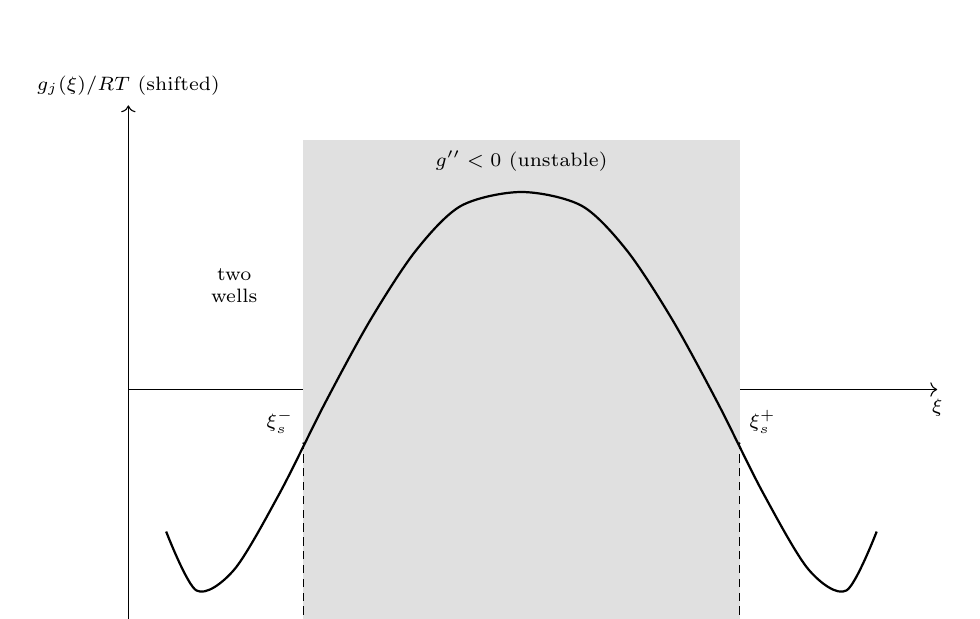
\begin{tikzpicture}[x=9.6cm,y=44cm]
% double-well free energy g(xi) for Omega=3RT (qualitative shape, normalized)
\draw[->] (-0.02,-0.069) -- (-0.02,0.082) node[above,font=\scriptsize] {$g_j(\xi)/RT$ (shifted)};
\draw[->] (-0.02,0) -- (1.05,0) node[below,font=\scriptsize] {$\xi$};
\foreach \xx in {0.25,0.5,0.75} {\draw (\xx,0.0015) -- (\xx,-0.0015) node[below,font=\scriptsize] {\xx};}
% spinodal band (g''<0) shading
\fill[black!12] (0.2113,-0.069) rectangle (0.7887,0.072);
\node[font=\scriptsize] at (0.5,0.066) {$g''<0$ (unstable)};
% the double well curve
\draw[thick] plot[smooth] coordinates {(0.03,-0.041) (0.07,-0.058) (0.12,-0.052) (0.18,-0.030) (0.24,-0.004) (0.3,0.020) (0.36,0.040) (0.42,0.053) (0.5,0.057) (0.58,0.053) (0.64,0.040) (0.7,0.020) (0.76,-0.004) (0.82,-0.030) (0.88,-0.052) (0.93,-0.058) (0.97,-0.041)};
% spinodal points
\fill (0.2113,-0.0155) circle (0.35pt) node[above left,font=\scriptsize] {$\xi_s^-$};
\fill (0.7887,-0.0155) circle (0.35pt) node[above right,font=\scriptsize] {$\xi_s^+$};
\draw[densely dashed] (0.2113,-0.069) -- (0.2113,-0.0155);
\draw[densely dashed] (0.7887,-0.069) -- (0.7887,-0.0155);
\node[font=\scriptsize,align=center] at (0.12,0.030) {two\\wells};
\end{tikzpicture}
\caption{격자기체 자유에너지 $g_j(\xi)$ (식~\eqref{eq:gxi}, $\Omega_j=3RT$; 신규 그림). $\Omega>2RT$ 면 가운데가
언덕이 되어 양쪽에 골짜기 둘 — 음영 띠($g''<0$, 식~\eqref{eq:gpp})가 변곡점 $\xi_s^\pm$ (spinodal, 식~\eqref{eq:spinodal})
사이의 불안정 구간이다. 이 곡률 부호 전환이 \S\ref{sec:hys} 의 비단조 전위 곡선과 분기 gap 을 낳는다.}
\label{fig:doublewell}
\end{figure}

\subsection{gap 의 닫힌 꼴 — 두 spinodal 의 전위 차}
\textbf{(a) 출발 — 비단조 평형 전위 곡선.} 평형 조건~\eqref{eq:eqcond}($\mu=\mu^0-sF(V-U)$, 배치 몫 자유에너지 기울기 $=$ 전기화학 구동력)에 의해 자유에너지~\eqref{eq:gxi} 의 1계 미분이 곧 평형 전위에 묶인다
($g_j'(\xi)=RT\ln[\xi/(1-\xi)]+\Omega_j(1-2\xi)=sF(V_\eq-U_j)$). 이를 $V_\eq$ 로 풀면
\begin{equation}
V_{\eq,j}(\xi)\;=\;U_j+\frac{RT}{sF}\ln\frac{\xi}{1-\xi}+\frac{\Omega_j}{sF}\,(1-2\xi),
\label{eq:Veq}
\end{equation}
이고 $\Omega_j>2RT$ 면 비단조다 — 방전은 $\xi\!\approx\!0$ 에서 상승 가지를 극대 $\xi_{s,j}^-$ 까지, 충전은 $\xi\!\approx\!1$
에서 극소 $\xi_{s,j}^+$ 까지 과주행하므로(전위 곡선의 극값이 $\dd V_\eq/\dd\xi=g_j''/sF=0$, 곧 spinodal 과 같은 점 —
그림~\ref{fig:hysloop}), 두 극값의 전위 차가 분기 gap 의 spinodal 상한이다. \textbf{(b) 연산 — spinodal 값 대입.}
식~\eqref{eq:spinodal} 의 $\xi_{s,j}^\pm=\tfrac12(1\pm u_j)$ 를 식~\eqref{eq:Veq} 의 두 비상수 항에 넣으면, logit 인자와
$(1-2\xi)$ 인자가 두 끝점에서 각각
\begin{equation}
\frac{\xi}{1-\xi}\bigg|_{\xi_{s,j}^\pm}=\frac{1\pm u_j}{1\mp u_j},
\qquad
(1-2\xi)\big|_{\xi_{s,j}^\pm}=\mp u_j
\label{eq:hyssub}
\end{equation}
— 곧 두 끝점에서 logit 인자가 서로 역수다. \textbf{(c) 중간식 — 극대에서 극소 빼기.} 극값 차를 적으면 상수항 $U_j$ 가
상쇄되고
\begin{align}
\Delta U_j^\hys
&=V_{\eq,j}(\xi_{s,j}^-)-V_{\eq,j}(\xi_{s,j}^+)\notag\\
&=\frac{RT}{sF}\Big[\ln\frac{1-u_j}{1+u_j}-\ln\frac{1+u_j}{1-u_j}\Big]
+\frac{\Omega_j}{sF}\big[u_j-(-u_j)\big]\notag\\
&=-\frac{4RT}{sF}\,\mathrm{artanh}\,u_j+\frac{2\Omega_j}{sF}\,u_j
\label{eq:hysdiff}
\end{align}
(둘째 줄의 두 로그가 부호 반대 같은 크기라 $\ln[(1-u)/(1+u)]-\ln[(1+u)/(1-u)]=-2\ln[(1+u)/(1-u)]=-4\,\mathrm{artanh}\,u$,
$\mathrm{artanh}\,u=\tfrac12\ln\tfrac{1+u}{1-u}$ 사용). \textbf{(d) 박스 — $s=+1$ 정리.}
\begin{equation}
\boxed{\;\Delta U_j^\hys
=\frac{2}{F}\Big[\Omega_j\,u_j-2RT\,\mathrm{artanh}\,u_j\Big],
\qquad u_j=\sqrt{1-\frac{2RT}{\Omega_j}}\;.}
\label{eq:dUhys}
\end{equation}
이것이 \code{func\_dU\_hys(T, Omega)} 의 \code{(2/F)*(Omega*u - 2*R*T*arctanh(u))} 이며, $\Omega\le2RT$ 면 $0$ 을
반환한다(제곱근 NaN 영역의 명시 분기). 부호 — 극대 $>$ 극소라 $\Delta U_j^\hys\ge0$ 이고, $\Omega_j\to2RT^+$ 에서
$u_j\to0$ 이라 Taylor 전개($\mathrm{artanh}\,u=u+u^3/3+\cdots$)로 $\Delta U_j^\hys\to\frac{8RT}{3F}u_j^3\to0$ 으로
연속이다($u_j^3\propto(T_{c,j}-T)^{3/2}$, $T_{c,j}=\Omega_j/2R$ — 임계온도에서 매끄럽게 소멸).

\subsection{방향별 분기 중심 $U_j^{\,d}$}
\textbf{(a) 출발 — 두 spinodal 끝점의 평균.} 식~\eqref{eq:hyssub} 의 두 대입값으로 두 끝점의 \emph{평균}을 적으면
로그 몫 합 $\ln\frac{1-u}{1+u}+\ln\frac{1+u}{1-u}=0$ 과 $(1-2\xi)$ 몫 합 $u+(-u)=0$ 이 둘 다 $0$ 이라
\begin{equation}
\tfrac12\big[V_{\eq,j}(\xi_{s,j}^-)+V_{\eq,j}(\xi_{s,j}^+)\big]=U_j
\label{eq:hyssym}
\end{equation}
— 분기는 $U_j$ 대칭이다. \textbf{(b)(c) 한 자유도로.} 이 대칭 위에서 실측 분기 중심을 방향별 한 자유도로 적으면(축소
인자 $\gamma_j$ 와 부분 cycle 인자 $h_{\eta,j}$ 를 곱해)
\begin{equation}
\boxed{\;U_j^{\,d}\;=\;U_j\;+\;\tfrac12\,\sigma_d\,h_{\eta,j}\,\gamma_j\,\Delta U_j^\hys\;.}
\label{eq:Ubranch}
\end{equation}
이것이 \code{func\_U\_branch(T, U\_j, Omega, gamma, sigma\_d, h\_eta)} 의
\code{U\_j + 0.5*sigma\_d*h\_eta*gamma*func\_dU\_hys(T, Omega)} 다. \textbf{(d) 부호.} 방전($\sigma_d=+1$)은 중심을
$+$ 쪽, 충전($\sigma_d=-1$)은 $-$ 쪽으로 옮겨 $U_j^{\dis}>U_j^{\chg}$(방전 전위가 충전보다 높다는 관측 일치).
$\gamma_j=1$ 이 spinodal 상한, $\gamma_j\to0$ 이 히스 소멸, $h_{\eta,j}$ 가 부분 cycle 보정(기본 $1$)이다.

코드는 전이당 상수인 분기 shift 만 필요하므로, 식~\eqref{eq:Ubranch} 의 $U_j$ 자리에 $0$ 을 넣어 shift 분
$\mathrm{hys\_shift}=\code{func\_U\_branch}(T_\rep,0,\Omega,\gamma,\sigma_d,h_\eta)$ 을 얻고, 배열 중심 $U_j$ 에 더한다:
\begin{equation}
\mathrm{center}=
\begin{cases}
U_j+\tfrac12\sigma_d h_{\eta,j}\gamma_j\Delta U_j^\hys(T_\rep) & \gamma_j\ne0 \text{ 이고 } \Omega_j>0\\[2pt]
U_j & \text{그 외(분기 없음)}.
\end{cases}
\label{eq:center}
\end{equation}
이 \code{center} 가 다음 절 평형 점유 $\xi_\eq$ 의 중심으로 들어간다. 평형 종의 \emph{모양} 자체는 방향 불변이고,
방향이 바꾸는 것은 이 중심의 위치(와 \S\ref{sec:tail} 의 꼬리 방향)뿐이다.

\begin{figure}[t]
\centering
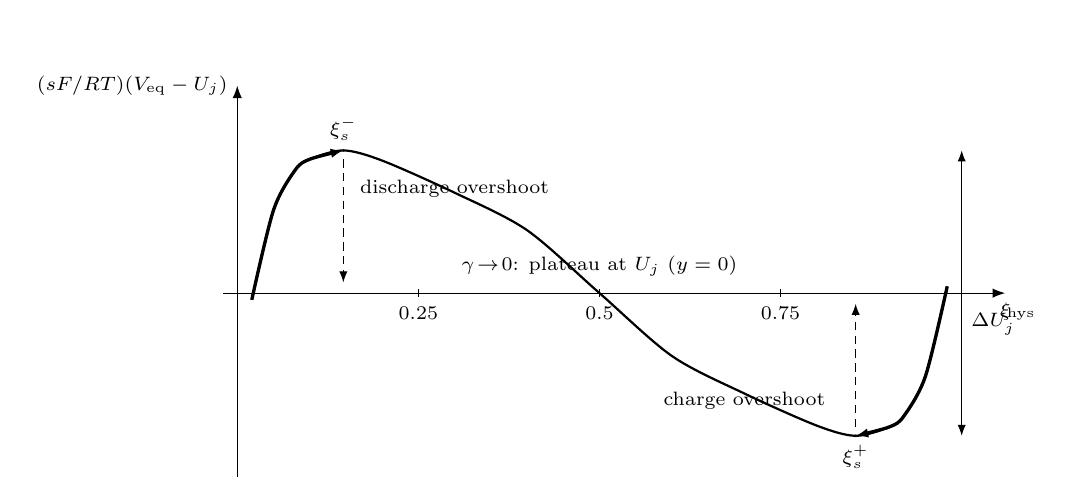
\begin{tikzpicture}[x=9.2cm,y=1.7cm]
\draw[-{Latex[length=1.6mm]}] (0,-1.45) -- (0,1.55) node[left,font=\scriptsize] {$(sF/RT)(V_\eq-U_j)$};
\draw[-{Latex[length=1.6mm]}] (-0.02,0) -- (1.06,0) node[below,font=\scriptsize] {$\xi$};
\foreach \xx in {0.25,0.5,0.75} {\draw (\xx,0.03) -- (\xx,-0.03) node[below,font=\scriptsize] {\xx};}
% non-monotone V_eq(xi) for Omega=4RT (qualitative)
\draw[thick] plot[smooth] coordinates {(0.02,-0.05) (0.05,0.62) (0.08,0.92) (0.1,1.00) (0.1464,1.066) (0.2,0.99) (0.3,0.75) (0.4,0.47) (0.5,0) (0.6,-0.47) (0.7,-0.75) (0.8,-0.99) (0.8536,-1.066) (0.9,-1.00) (0.92,-0.92) (0.95,-0.62) (0.98,0.05)};
\fill (0.1464,1.066) circle (0.5pt) node[above,font=\scriptsize] {$\xi_s^-$};
\fill (0.8536,-1.066) circle (0.5pt) node[below,font=\scriptsize] {$\xi_s^+$};
\draw[{Latex[length=1.4mm]}-{Latex[length=1.4mm]}] (1.0,-1.066) -- (1.0,1.066) node[pos=0.4,right,font=\scriptsize] {$\Delta U_j^\hys$};
% discharge overshoot path (rising branch up to xi_s^-)
\draw[-{Latex[length=1.6mm]},very thick] plot[smooth] coordinates {(0.02,-0.05) (0.05,0.62) (0.08,0.92) (0.1,1.00) (0.1464,1.066)};
\draw[-{Latex[length=1.4mm]},densely dashed] (0.1464,1.0) -- (0.1464,0.08);
\node[font=\scriptsize] at (0.30,0.78) {discharge overshoot};
% charge overshoot path
\draw[-{Latex[length=1.6mm]},very thick] plot[smooth] coordinates {(0.98,0.05) (0.95,-0.62) (0.92,-0.92) (0.9,-1.00) (0.8536,-1.066)};
\draw[-{Latex[length=1.4mm]},densely dashed] (0.8536,-1.0) -- (0.8536,-0.08);
\node[font=\scriptsize] at (0.70,-0.80) {charge overshoot};
\node[font=\scriptsize] at (0.5,0.20) {$\gamma\!\to\!0$: plateau at $U_j$ ($y=0$)};
\end{tikzpicture}
\caption{비단조 평형 전위 $V_\eq(\xi)$(식~\eqref{eq:Veq}, $\Omega_j=4RT$)와 과주행(v7-11 유래). 방전(굵은 경로,
좌상)은 극대 $\xi_s^-$ 까지, 충전(우하)은 극소 $\xi_s^+$ 까지 과주행해 중심이 갈라진다. 두 극값 차가 spinodal 상한
gap $\Delta U_j^\hys$(식~\eqref{eq:dUhys}), 실측 분기는 $\gamma_j$ 만큼 안쪽(식~\eqref{eq:Ubranch}). $\gamma\to0$
가역 한계에서 두 경로가 $y=0$ plateau 로 합쳐진다.}
\label{fig:hysloop}
\end{figure}

\subsection{LCO order--disorder 와 MIT 2상역 — 같은 정규용액 틀}\label{sec:lco-hys}
\S\ref{sec:hys} 의 격자기체$\cdot$정규용액 틀은 ``동등한 자리에 리튬이 차고 빈다''는 가정만 쓰므로, 그 가정이 서는 LCO
양극에도 그대로 적용된다 — $\Omega_j$ 의 \emph{값}만 LCO 의 상전이가 정한다. LCO 에서 $\Omega_j>2RT$ 의 상분리(따라서
2상 plateau$\cdot$히스테리시스)를 낳는 자리는 표~\ref{tab:lco-staging} 의 세 전이 모두에 대응한다.

\textbf{(T2$\cdot$T3) order--disorder.} $x\approx0.5$ 부근에서 $\mathrm{Li}_x\mathrm{CoO_2}$ 는 점유 리튬과 빈자리가
교대로 정렬하는 monoclinic 초격자(질서상)를 이룬다 — 이 정렬은 정규용액의 $\Omega>0$(동종 이웃 인력으로 가운데를 위로
미는 이중웰, 식~\eqref{eq:gxi})이 만드는 상분리의 LCO 사례다. 한 쌍 전이(T2 $\sim$4.05 V hex$\to$monoclinic,
T3 $\sim$4.17 V monoclinic$\to$hex)가 식~\eqref{eq:spinodal} 의 spinodal 문턱 $\Omega_j>2RT$ 를 넘어 두 개의 좁은
peak 로 갈라진다. 정렬의 charge-order 엔트로피 변화($\approx$0.47 J/K\,mol@$x{=}\tfrac12$, $\approx$1.49 J/K\,mol@$x{=}\tfrac23$
[tier A, Motohashi~\cite{motohashi2009}])가 표~\ref{tab:lco-staging} 의 config 주도 $\Delta S$ 의 출처다.

\textbf{(T1) MIT 2상역.} $x\approx0.75$--$0.94$ 의 절연체$\to$금속 천이(MIT)도 2상 공존역이다(전위 plateau$\sim$3.9 V).
이 구간 역시 식~\eqref{eq:dUhys}$\cdot$\eqref{eq:Ubranch} 의 spinodal gap$\cdot$분기 중심을 그대로 받는다 — 곧 LCO 의
MIT plateau 도 $\Delta U_j^\hys$ 와 $\gamma_j$ 로 충방전 히스를 적는다. 다만 MIT 에는 격자기체 config 만으로 닫히지 않는
\emph{전자 자유도}(전도 전자의 상태밀도 변화)가 있어, 엔트로피에 흑연엔 없는 항이 하나 더 붙는다 — 이것이
\S\ref{sec:lco-electronic} 의 전자 엔트로피 항이다. 여기서는 ``MIT 의 구조적 2상역은 정규용액 틀로, 전자 자유도는 별도
항으로'' 두 몫을 분리한다는 점만 못박는다(이중계산 방지의 출발).

\textbf{도핑 보정(우리 시료).} Al$^{3+}$/Mg$^{2+}$ 비-redox 치환은 Co redox 와 전자항을 보존하되 order--disorder$\cdot$MIT
상전이를 \emph{억제}한다 — 정규용액 틀에서 이는 $\Omega_j$ 를 $2RT$ 쪽으로 낮춰(또는 유효 폭을 넓혀, 식~\eqref{eq:weff})
peak 를 smear 하고 $U_j$ 를 미세 shift 시키는 것으로 들어온다. 흑연 \code{GRAPHITE\_STAGING\_LIT} 가 초기값이고 폭이
피팅 대상이었듯, pure-LCO 의 $\Omega_j$ 가 초기값이고 도핑에 따른 폭$\cdot$shift 는 우리 데이터로 피팅한다.

% ====================================================================
\section{폭과 평형 점유 $\xi_\eq$ (N4, N5)}\label{sec:width}
% ====================================================================
중심이 정해지면 코드는 폭 $w_j$ 와 평형 점유 $\xi_{\eq,j}$ 를 평가한다. 이 둘이 평형 종(다음 절의 peak)의 모양을
결정한다. 평형 등온선은 \S\ref{sec:center} 의 평형 조건을 정$\cdot$역 속도의 균형으로 회수하면 logistic 으로 닫히는데,
그 회수가 이 절의 핵심 유도다 — 먼저 폭을 세운 뒤 logistic 을 detailed balance 에서 끌어낸다.

\subsection{폭 $w_j$ — 이상 극한과 옵션}
평형 점유의 폭 척도는 이상 극한에서 $w_j=n_jRT/F$ 다($n_j$ 는 폭 다중도): 아래 \S\ref{sec:width} logistic 유도의
중심 기울기 $\dd\xi_\eq/\dd V|_{1/2}=sF/(4RT)$ 가 폭 척도 $RT/F$ 를 정의하고, 폭 다중도 $n_j$ 로 일반화하면
\begin{equation}
w_j=\frac{n_jRT}{F}\qquad(\text{기본 폭}),
\label{eq:wbase}
\end{equation}
코드 \code{func\_w(T, n)} 의 \code{n*R*T/F}
가 이것이고, 전이 dict 가 \code{'w'} 를 직접 주면 $n_j=w_jF/(RT)$ 로 역산해(\code{\_n\_factor}) 같은 식에 넣는다.
상호작용이 종을 좁히는 옵션 유효 폭은, 비단조 등온선~\eqref{eq:Veq} 의 중심 기울기를 이상 logistic 의 중심 기울기와
같다고 둔 데서 온다 — $sF\,\dd V_\eq/\dd\xi|_{1/2}=4RT-2\Omega_j$ 와 $4Fw^\eff_j$ 를 같다고 풀면($s$ 부호는 양변 공통이라 상쇄)
\begin{equation}
w_j^\eff=\frac{RT}{F}\Big(1-\frac{\Omega_j}{2RT}\Big),
\label{eq:weff}
\end{equation}
이며 $\Omega_j\to2RT$ 에서 $0$ 으로 가므로 코드는 $\mathrm{floor\_frac}\cdot RT/F$ 하한으로 클립한다(\code{func\_w\_eff},
기본 \code{w\_eff\_floor\_frac}$=0.05$). 이 좁힘은 명시적으로 \code{use\_w\_eff} 를 켤 때만 적용되고, 기본은
$w_j=n_jRT/F$ 다(\code{\_width}).

\subsection{평형 점유 $\xi_\eq$ — logistic 의 유도}
\textbf{(a) 출발 — Eyring 속도식과 비대칭 장벽.} 활성화 장벽 $\Delta G_a$ 이상을 갖출 확률은 Boltzmann 분포
$\propto e^{-\Delta G_a/RT}$ 이고, 전이상태 이론의 시도 빈도 $k_0=k_BT/h$ 를 곱하면 Eyring 속도식
$k\simeq k_0e^{-\Delta G_a/RT}$ 다(그림~\ref{fig:barrier})\cite{eyring1935}. 구동력 $\mathcal A_j=sF(V_n-U_j)$ 가 정$\cdot$역 장벽을
비대칭 이동시켜(분율 위치 $\chi$ — 비평형 열역학 기반 전하전달 동역학의 표준 분해\cite{bazant2013}), 자리당 정$\cdot$역 속도가
\begin{equation}
r_j^+=k_0\,e^{-(\Delta G_{a,j}-\chi\mathcal A_j)/RT},\qquad
r_j^-=k_0\,e^{-(\Delta G_{a,j}+(1-\chi)\mathcal A_j)/RT}.
\label{eq:bv}
\end{equation}
\textbf{(b) 연산 — 비를 취해 detailed balance.} 두 속도의 비를 취하면 $k_0,e^{-\Delta G_a/RT}$ 가 약분되고 지수의
$\chi$ 가 상쇄되어($\chi\mathcal A+(1-\chi)\mathcal A=\mathcal A$)
\begin{equation}
\frac{r_j^+}{r_j^-}=\exp\!\Big[\frac{\chi\mathcal A_j+(1-\chi)\mathcal A_j}{RT}\Big]=\exp\!\Big[\frac{\mathcal A_j}{RT}\Big]
\label{eq:db}
\end{equation}
— 평형비가 $\chi$ 와 무관한 Boltzmann 비라는 detailed balance 다($\chi+(1-\chi)=1$ 합-1 제약이 강제한 결과). 운동
방정식은 정방향이 찬 자리($1-\xi$)에서, 역방향이 빈 자리($\xi$)에서 출발하므로
$\dd\xi/\dd t=r^+(1-\xi)-r^-\xi=k_j(\xi_\eq-\xi)$($k_j\equiv r^++r^-$). \textbf{(c) 중간식 — 정지점에서 logit.}
정지점 $\dd\xi/\dd t=0$ 에서 $r^+(1-\xi_\eq)=r^-\xi_\eq$(정$\cdot$역 플럭스의 교점 — 그림~\ref{fig:flux}), 곧
비 식~\eqref{eq:db} 로
\begin{equation}
\frac{\xi_\eq}{1-\xi_\eq}=e^{\mathcal A_j/RT}=e^{sF(V_n-U_j)/RT}
\quad\Longrightarrow\quad
\xi_\eq=\frac{1}{1+e^{-sF(V_n-U_j)/RT}}
\label{eq:logisticsolve}
\end{equation}
(둘째 식은 분모$\cdot$분자를 $e^{\mathcal A/RT}$ 로 나눈 것). \textbf{(d) 박스 — 폭 다중도$\cdot$방향 부호 일반화.}
폭 척도 $w_j=n_jRT/F$(식~\eqref{eq:wbase})로 묶고 방향 부호 $\sigma_d$ 와 분기 중심 $U_j^{\,d}$ 로 일반화하면
\begin{equation}
\boxed{\;\xi_{\eq,j}(V,T)=\frac{1}{1+\exp\!\big[-\sigma_d(V-U_j^{\,d})/w_j\big]}\;.}
\label{eq:xieq}
\end{equation}
열역학은 detailed balance~\eqref{eq:db} 한 곳으로만 들어왔다 — logistic 은 속도식의 정지점에서 \emph{유도된}
평형이다. 방향 부호가 logistic 인자의 부호로 들어가는 것이 \code{func\_ksi\_eq(T, V\_n, U, n, s)} 의
$z=\sigma_d(V_\work-U_j^{\,d})/w_j$(폭은 \code{func\_w}$(T,n)$)이며, 코드는 오버플로 방지를 위해 $z\ge0$ 과 $z<0$ 을
갈라 평가한다(\code{np.where(z>=0, 1/(1+e\^{-z}), e\^{z}/(1+e\^{z}))} — 수학적으로 동일). 여기서 평가 전위는
내부 전위 $V_n$ 이 아니라 \S\ref{sec:pol} 의 작업 격자 $V_\work$ 다 — 코드 호출 \code{func\_ksi\_eq(T\_work,
V\_work, center, n\_j, sigma\_d)} 에서 함수의 \code{V\_n} 인자 자리에 $V_\work$ 가 들어간다(평형$\cdot$동역학은
$V_\work$ 위에서 풀고 출력만 $V_n$ 으로 역보간하는 규약, 식~\eqref{eq:vwork}). 호출 시 중심 $U_j^{\,d}$ 는
식~\eqref{eq:center} 의 \code{center}(분기 있으면 분기 중심, 없으면 $U_j$)다.

\begin{figure}[t]
\centering
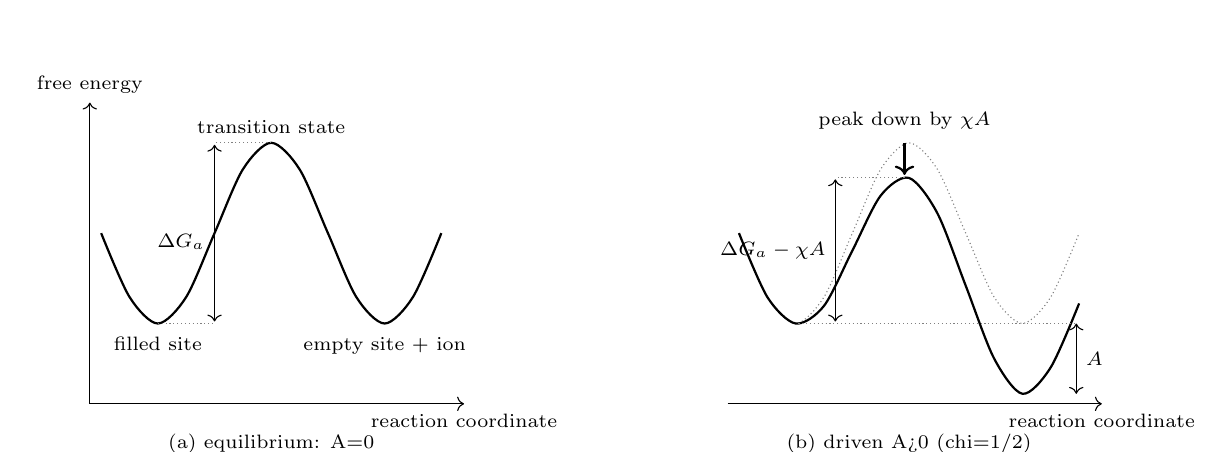
\begin{tikzpicture}[x=0.72cm,y=2.55cm]
% ---- (a) equilibrium landscape ----
\draw[->] (-0.2,-0.3) -- (6.4,-0.3) node[below,font=\scriptsize] {reaction coordinate};
\draw[->] (-0.2,-0.3) -- (-0.2,1.2) node[above,font=\scriptsize] {free energy};
\draw[thick] plot[smooth] coordinates {(0,0.55) (0.5,0.232) (1,0.1) (1.5,0.232) (2,0.55) (2.5,0.868) (3,1.0) (3.5,0.868) (4,0.55) (4.5,0.232) (5,0.1) (5.5,0.232) (6,0.55)};
\node[below,font=\scriptsize] at (1,0.08) {filled site};
\node[below,font=\scriptsize] at (5,0.08) {empty site + ion};
\node[above,font=\scriptsize] at (3,1.0) {transition state};
\draw[densely dotted,gray] (1,0.1) -- (2.0,0.1);
\draw[densely dotted,gray] (3,1.0) -- (2.0,1.0);
\draw[<->] (2.0,0.11) -- (2.0,0.99) node[pos=0.45,left,font=\scriptsize] {$\Delta G_a$};
\node[font=\scriptsize] at (3,-0.5) {(a) equilibrium: A=0};
\begin{scope}[xshift=8.1cm]
% ---- (b) driven landscape: A>0, chi=1/2 ----
\draw[->] (-0.2,-0.3) -- (6.4,-0.3) node[below,font=\scriptsize] {reaction coordinate};
\draw[densely dotted,thin,gray] plot[smooth] coordinates {(0,0.55) (0.5,0.232) (1,0.1) (1.5,0.232) (2,0.55) (2.5,0.868) (3,1.0) (3.5,0.868) (4,0.55) (4.5,0.232) (5,0.1) (5.5,0.232) (6,0.55)};
\draw[thick] plot[smooth] coordinates {(0,0.550) (0.5,0.232) (1,0.100) (1.5,0.188) (2,0.463) (2.5,0.737) (3,0.825) (3.5,0.649) (4,0.288) (4.5,-0.074) (5,-0.250) (5.5,-0.118) (6,0.200)};
\draw[->,thick] (2.92,1.0) -- (2.92,0.84) ;
\node[above,font=\scriptsize] at (2.92,1.02) {peak down by $\chi A$};
\draw[densely dotted,gray] (1.05,0.1) -- (1.7,0.1);
\draw[densely dotted,gray] (2.92,0.828) -- (1.7,0.828);
\draw[<->] (1.7,0.11) -- (1.7,0.818) node[pos=0.5,left,font=\scriptsize] {$\Delta G_a-\chi A$};
\draw[densely dotted,gray] (1.05,0.1) -- (5.95,0.1);
\draw[<->] (5.95,0.1) -- (5.95,-0.25) node[pos=0.5,right,font=\scriptsize] {$A$};
\node[font=\scriptsize] at (3,-0.5) {(b) driven A>0 (chi=1/2)};
\end{scope}
\end{tikzpicture}
\caption{활성화 장벽 그림(신규). (a) 평형 — 두 골짜기 같은 높이, 속도는 Eyring 식. (b) 구동력 $\mathcal A_j$ 가
도착 골짜기를 내리면 정방향 장벽 $\Delta G_a-\chi\mathcal A$, 역방향 $\Delta G_a+(1-\chi)\mathcal A$ 로 비대칭 이동
(식~\eqref{eq:bv}; 두 속도의 비가 식~\eqref{eq:db} detailed balance). 점선은 (a). 온도는 분모 $RT$ 로 진입.
이 그림이 식~\eqref{eq:xieq} logistic 과 \S\ref{sec:lag} 의 $L_q$ 두 결과의 공통 출발점이다.}
\label{fig:barrier}
\end{figure}

\begin{figure}[t]
\centering
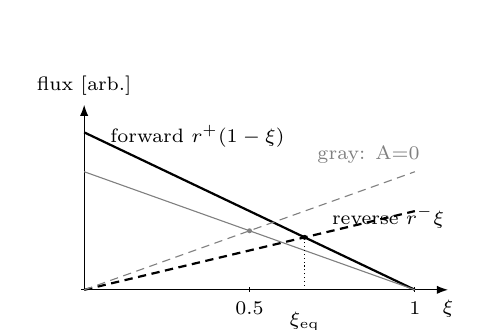
\begin{tikzpicture}[x=4.2cm,y=1.0cm]
\draw[-{Latex[length=1.4mm]}] (0,0) -- (0,2.35) node[above,font=\scriptsize] {flux [arb.]};
\draw[-{Latex[length=1.4mm]}] (-0.01,0) -- (1.1,0) node[below,font=\scriptsize] {$\xi$};
\foreach \xx in {0.5,1} {\draw (\xx,0.03) -- (\xx,-0.03) node[below,font=\scriptsize] {\xx};}
% forward r+ (1-xi): decreasing line from 2 to 0
\draw[thick] (0,2) -- (1,0);
% reverse r- xi: increasing line from 0 to 1
\draw[thick,densely dashed] (0,0) -- (1,1);
% A=0 pair (gray)
\draw[gray] (0,1.5) -- (1,0);
\draw[gray,densely dashed] (0,0) -- (1,1.5);
% intersection black: 2(1-xi)=xi -> xi=2/3
\draw[densely dotted] (0.6667,0) -- (0.6667,0.6667);
\fill (0.6667,0.6667) circle (0.9pt);
\node[below,font=\scriptsize] at (0.6667,-0.16) {$\xi_\eq$};
\fill[gray] (0.5,0.75) circle (0.9pt);
\node[right,font=\scriptsize] at (0.05,1.95) {forward $r^+(1-\xi)$};
\node[right,font=\scriptsize] at (0.72,0.92) {reverse $r^-\xi$};
\node[gray,font=\scriptsize] at (0.86,1.72) {gray: A=0};
\end{tikzpicture}
\caption{정지점 유도(신규). 정방향 플럭스 $r^+(1-\xi)$(감소 직선)와 역방향 $r^-\xi$(증가 직선)의 교점이 정지점
$\xi_\eq$(식~\eqref{eq:logisticsolve}). $\mathcal A>0$($r^+=2r^-$, 검정)이면 $\xi_\eq=2/3$, $\mathcal A=0$
(회색)이면 $\tfrac12$ — detailed balance(식~\eqref{eq:db})가 평형을 정한다.}
\label{fig:flux}
\end{figure}

\begin{signbox}
\textbf{부호.} 방전 $\sigma_d=+1$: $V\!\uparrow\Rightarrow z\!\uparrow\Rightarrow\xi_\eq\!\uparrow$ — 전위를 올리면
탈리튬화 진행이 는다(규약 일치). 충전 $\sigma_d=-1$: $V\!\uparrow\Rightarrow z\!\downarrow\Rightarrow\xi_\eq\!\downarrow$.
극한 — $V\gg U_j^{\,d}\Rightarrow\xi_\eq\to1$(방전), $V\ll U_j^{\,d}\Rightarrow0$, $V=U_j^{\,d}\Rightarrow\tfrac12$
(전이 중심). $w_j=RT/F=25.7$ mV($25^\circ$C).
\end{signbox}

\subsection{같은 결과의 분포 관점 — $\xi_\eq$ 는 평형 점유 확률 분포}\label{sec:dist}
앞에서 $\xi_\eq$ 는 두 경로로 나왔다 — (i) kinetic: 속도식 정지점에서 detailed balance~\eqref{eq:db}(식~\eqref{eq:logisticsolve}),
(ii) thermo: 자유에너지 최소화 $g_j'(\xi)=sF(V_\eq-U)$(식~\eqref{eq:Veq}). 이 둘은 사실 \emph{하나의 분포}의 두 얼굴이다.
이 소절은 그 분포 관점을 한 단락으로 닫는다 — 결과식$\cdot$부호$\cdot$코드는 불변이고, $\xi_\eq$ 가 ``무엇인지''의 통계역학적
정체만 더한다. 이 정체가 \S\ref{sec:lco-electronic} 의 LCO 전자 엔트로피(전도 전자 Fermi--Dirac 분포)와 \emph{같은
언어}라, 두 곳을 한 그림으로 묶는다.

\textbf{(a) 출발 — 단일 자리 grand-canonical 점유.} 한 전이의 \emph{한} 흡착 자리를 떼어 보자 — 그 자리는 비었거나
($\varepsilon=0$) 리튬 1개가 들었다($\varepsilon=\Delta\mu$, 자리 점유의 자유에너지 비용). 두 미시상태의
grand-canonical 분배함수는
\begin{equation}
Z\;=\;1+e^{-\beta\,\Delta\mu},\qquad \beta\equiv\frac{1}{k_BT},\quad
\Delta\mu\equiv\varepsilon_\mathrm{occ}-\mu_\mathrm{Li}
\label{eq:partfn}
\end{equation}
($1$ = 빈 자리, $e^{-\beta\Delta\mu}$ = 점유 자리의 Boltzmann 가중). \textbf{(b) 연산 — 평균 점유.} 식~\eqref{eq:partfn}
의 $Z$ 로 점유 상태 가중을 나누면 점유 확률(평균 점유)이다:
\begin{equation}
\langle n\rangle\;=\;\frac{e^{-\beta\Delta\mu}}{1+e^{-\beta\Delta\mu}}
\;=\;\frac{1}{1+e^{+\beta\Delta\mu}}.
\label{eq:fermifn}
\end{equation}
\textbf{(c) 같은 식 — logistic 과의 일치.} 전기화학 구동력이 자리 점유 비용을 정한다 — 1몰 기준으로
$\Delta\mu=-sF(V-U_j)$(식~\eqref{eq:eqcond} 의 $\mu_\mathrm{Li}=\mu^0-sF(V-U)$ 를 단일 자리 점유에 적용)이고, 이때
지수 $\beta\Delta\mu$ 는 몰당 형태로 $\Delta\mu/(RT)=-sF(V-U_j)/(RT)=-s(V-U_j)/w_j$($w_j\equiv RT/F$, 이상 극한)다
($\beta$ 의 자리당 $k_BT$ 가 몰당 $RT$ 로, 자리당 전하 $e$ 가 몰당 $F$ 로 한꺼번에 환산 — 비는 불변). 따라서
식~\eqref{eq:fermifn} 은 $\langle n\rangle=1/(1+e^{-s(V-U_j)/w_j})$ 곧 식~\eqref{eq:logisticsolve}$\cdot$\eqref{eq:xieq}
의 $\xi_\eq$ 와 \emph{같은 식}이다. 곧 \emph{$\xi_\eq$ 는 격자기체의 평형 점유 확률 분포 그 자체}이며, 이것이
Fermi--Dirac 함수와 같은 꼴인 것은 ``한 자리에 입자 0 또는 1''이라는 배타적 점유를 공유하기 때문이다.

\textbf{(d) 두 경로의 통합.} 이 분포 관점이 (i)(ii)를 묶는다 — kinetic 경로는 ``정$\cdot$역 플럭스가 균형을 이루는 정지
점유''(식~\eqref{eq:db}), thermo 경로는 ``자유에너지를 최소화하는 점유''인데, 둘 다 \emph{같은 grand-canonical 평형
점유 분포}(식~\eqref{eq:fermifn})에 도달한다. $\Omega=0$(이상 격자기체)이면 분포가 정확히 Fermi-함수형이고, $\Omega>0$
이면 평균장 자리 비용 $\Delta\mu$ 에 $-\Omega(1-2\xi)$ 가 더해져(식~\eqref{eq:mu}) 자기무모순 분포가 된다 — 그
비단조성이 \S\ref{sec:hys} 의 히스이고, 그 분포의 변곡(spinodal)이 식~\eqref{eq:spinodal} 이다. 곧 ``점유 분포''
한 언어가 평형 중심$\cdot$폭$\cdot$히스$\cdot$logistic 을 한 줄에 꿴다.

\begin{keybox}
\textbf{분포 다리.} $\xi_\eq$ = 평형 점유 확률 분포(식~\eqref{eq:fermifn}, $Z=1+e^{-\beta\Delta\mu}$). 이 ``입자 0/1
배타 점유의 Fermi-함수형'' 언어가 \S\ref{sec:lco-electronic} 의 LCO \emph{전자} 엔트로피(전도 전자의 Fermi--Dirac
분포 $f(E)=1/(1+e^{\beta(E-E_F)})$)와 동형이다 — 흑연의 \emph{리튬 자리} 점유 분포와 LCO 의 \emph{전자 준위} 점유
분포가 같은 통계로 닫힌다. 이 다리가 LCO 전자 엔트로피 절을 흑연 forward 틀 안으로 끌어들인다.
\end{keybox}

그림~\ref{fig:logistic} 가 $\xi_\eq$ 와 그 미분(다음 절의 종)을 함께 보인다. 다음 절은 이 종이 평형 peak 임을 닫는다.

\begin{figure}[t]
\centering
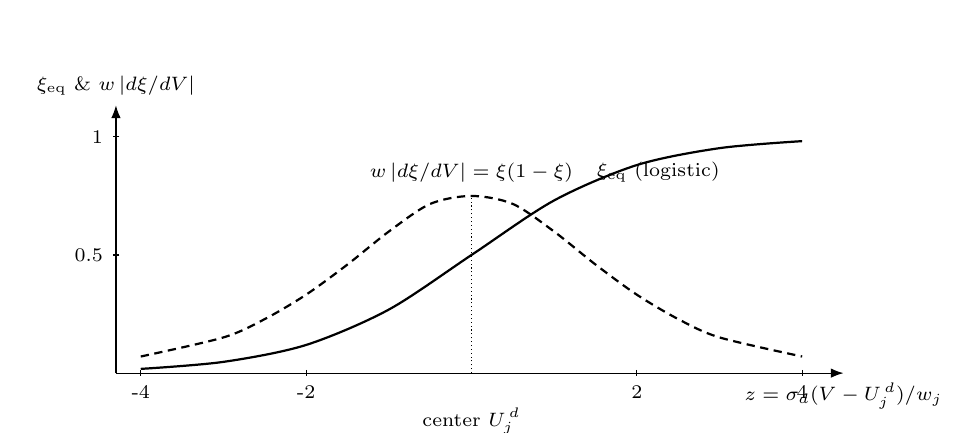
\begin{tikzpicture}[x=1.05cm,y=1.0cm]
% left axis: xi_eq (S-curve), right: dxi/dV bell — shared z-axis
\draw[-{Latex[length=1.6mm]}] (-4.3,0) -- (4.5,0) node[below,font=\scriptsize] {$z=\sigma_d(V-U_j^{\,d})/w_j$};
\draw[-{Latex[length=1.6mm]}] (-4.3,0) -- (-4.3,3.4) node[above,font=\scriptsize] {$\xi_\eq$ \&\ $w\,|d\xi/dV|$};
\foreach \xx in {-4,-2,2,4} {\draw (\xx,0.04) -- (\xx,-0.04) node[below,font=\scriptsize] {\xx};}
\draw (-4.26,3.0) -- (-4.34,3.0) node[left,font=\scriptsize] {1};
\draw (-4.26,1.5) -- (-4.34,1.5) node[left,font=\scriptsize] {0.5};
% xi_eq = 1/(1+e^-z) scaled by 3
\draw[thick] plot[smooth] coordinates {(-4,0.0537) (-3,0.1429) (-2,0.3577) (-1,0.8068) (0,1.5) (1,2.1932) (2,2.6423) (3,2.8571) (4,2.9463)};
\node[right,font=\scriptsize] at (1.4,2.55) {$\xi_\eq$ (logistic)};
% derivative xi(1-xi) max 0.25 scaled by 12 -> max 3
\draw[densely dashed,thick] plot[smooth] coordinates {(-4,0.211) (-3,0.4534) (-2.5,0.6864) (-2,0.9963) (-1.5,1.3792) (-1,1.7976) (-0.5,2.1487) (0,2.25) (0.5,2.1487) (1,1.7976) (1.5,1.3792) (2,0.9963) (2.5,0.6864) (3,0.4534) (4,0.211)};
\node[font=\scriptsize] at (0,2.55) {$w\,|d\xi/dV|=\xi(1-\xi)$};
\draw[densely dotted] (0,0)--(0,2.25);
\node[below,font=\scriptsize] at (0,-0.32) {center $U_j^{\,d}$};
\end{tikzpicture}
\caption{평형 점유와 그 미분(v7-11 유래). 실선 $=\xi_\eq$ logistic(식~\eqref{eq:xieq}), 파선 $=$ 폭으로 규격화한
미분 $w_j|d\xi_\eq/dV|=\xi_\eq(1-\xi_\eq)$ — $z=0$(중심 $U_j^{\,d}$)에서 최대 $\tfrac14$ 인 종 모양. 이 종이
다음 절의 평형 peak 이고, 방향에 불변(양수)이다.}
\label{fig:logistic}
\end{figure}

% ====================================================================
\section{LCO 전자 엔트로피 항 — 흑연엔 없는 성분 (N5+)}\label{sec:lco-electronic}
% ====================================================================
지금까지 $\Delta S_{\rxn,j}$ 는 배치(configurational)와 격자진동(vibrational) 두 몫이면 닫혔다 — 흑연은 그 둘로 충분하다.
LCO 양극은 한 몫이 더 있다: \emph{전자(electronic) 엔트로피}. 흑연은 충방전 동안 전자구조 변화가 미미해(반금속$\cdot$전도성
변화 작음) 전자항을 무시할 수 있지만, LCO 는 $x\!\downarrow$ 에서 절연체$\to$금속 천이(MIT)를 겪어 Fermi 준위 상태밀도
$g(E_F)$ 가 $0$ 에서 유한값으로 켜진다 — 이 전자 분포의 변화가 엔트로피에 들어온다. \textbf{이 대비(흑연=전자항 0,
LCO=MIT 로 필수)가 통합 챕터의 교육 가치다.} 이 절은 그 항을, \S\ref{sec:dist} 의 ``점유 분포'' 언어를 전자 준위로
옮겨 Fermi--Dirac 분포에서 한 단계씩 유도하고, 1차 문헌에 연속 곡선이 없는 빈자리를 ★\emph{MIT-logistic 게이트}라는
모델 가정으로 메우되 그 가정을 물리로 정당화한다.

\subsection{왜 흑연엔 없고 LCO엔 있나 — MIT 의 물리}\label{sec:lco-why}
삽입 반응의 전체 엔트로피 변화는 ``리튬 자리가 어떻게 배열되나''(config)$\cdot$``격자가 어떻게 진동하나''(vib)$\cdot$
``전자가 어떤 준위를 어떻게 점유하나''(electronic) 세 자유도의 합이다. 흑연에서는 셋째 몫이 작다 — 흑연$\cdot$
$\mathrm{LiC_6}$ 모두 전도성이 좋아 충방전 동안 $g(E_F)$ 가 크게 바뀌지 않으므로, 전자 분포의 엔트로피 \emph{변화}가
거의 없다. LCO 는 다르다: $x{=}1$($\mathrm{LiCoO_2}$)은 Co$^{3+}$($t_{2g}^6$ low-spin, 닫힌 껍질)라 \emph{전기 절연체}
($g(E_F)\!\approx\!0$)이고, 탈리튬화로 $x$ 가 $\sim$0.94 아래로 내려가면 Co$^{4+}$ 정공이 생겨 $t_{2g}$ 띠에 전도 전자가
열려 \emph{금속}이 된다($g(E_F)\!\to\!$유한)\cite{menetrier1999,motohashi2009}. 이 절연체$\to$금속 천이(MIT)가 $x\approx0.75$--$0.94$
의 2상역에서 일어나며(\S\ref{sec:lco-hys} 의 T1), 그 구간에서만 전자 분포가 켜지므로 전자 엔트로피 \emph{변화}도 그
구간에 국소한다. 곧 ``전자항이 켜지는 게이트''는 MIT 의 직접 결과다.

\subsection{Fermi--Dirac 에서 Sommerfeld 전자 엔트로피로 — 유도}\label{sec:lco-Se}
\textbf{(a) 출발 — 전도 전자의 Fermi--Dirac 분포.} \S\ref{sec:dist} 에서 흑연 리튬 자리의 평형 점유가 Fermi-함수형
이었듯, LCO 의 전도 전자도 에너지 준위 $E$ 를 Fermi--Dirac 분포로 점유한다:
\begin{equation}
f(E)=\frac{1}{1+e^{(E-E_F)/k_BT}}
\label{eq:fd}
\end{equation}
($E_F$ = Fermi 준위). 입자 0/1 배타 점유라는 구조가 식~\eqref{eq:fermifn} 의 리튬 자리 점유와 \emph{같다} — 다만 자리가
``리튬 흡착 자리''가 아니라 ``전자 에너지 준위''다. \textbf{(b) 연산 — 분포에서 엔트로피.} 이 분포의 엔트로피는 두 상태
점유의 정보 엔트로피를 모든 준위에 합한 것이다($-k_B\sum[f\ln f+(1-f)\ln(1-f)]$, 식~\eqref{eq:fd} 를 자리당 점유로 본
\S\ref{sec:hys} 의 $S_\mathrm{mix}$ 와 같은 꼴). 축퇴 전자기체($k_BT\!\ll\!E_F$)에서 이 합은 Fermi 준위 근방의 좁은
열폭($\sim k_BT$)에만 기여가 살아 Sommerfeld 전개로 닫힌다. \textbf{(c) 중간식 — Sommerfeld 전개로 $C_e$, 그리고 적분으로 $S_e$.}
\emph{여기서 한 가정을 명시한다} — 표준 Sommerfeld 처방대로 상태밀도 $g(E)$ 를 그 좁은 열폭($\sim k_BT$) 안에서
$E_F$ 근방의 \emph{상수} $g(E_F)$ 로 동결한다($g(E)\approx g(E_F)$). 이 동결이 정당한 까닭은, 적분에 기여하는 띠가
폭 $\sim k_BT$ 로 좁고 축퇴 극한 $k_BT\!\ll\!E_F$ 에서는 그 좁은 창 안에서 $g(E)$ 의 에너지 의존이 선도 차수로
무시되기 때문이다 — 이것이 금속 전자기체의 표준 Sommerfeld 근사다. 이 동결 아래 표준 Sommerfeld 적분
$\int(-\partial f/\partial E)(E-E_F)^2\dd E=\tfrac{\pi^2}{3}(k_BT)^2$ 가
전자 \emph{비열}을 먼저 닫는다 — 내부에너지 $U_e=\int E\,g(E)f\,\dd E$ 의 온도 미분에서 $g(E_F)$ 를 적분 밖으로 빼
이 적분을 대입하면
$C_e=\partial U_e/\partial T=\tfrac{\pi^2}{3}k_B^2T\,g(E_F)$($T$-선형 전자 비열, 금속의 표준 결과)다. 엔트로피는 이
비열을 $S_e=\int_0^T (C_e/T')\,\dd T'$ 로 적분한 것이고, $C_e/T'=\tfrac{\pi^2}{3}k_B^2g(E_F)$ 가 $T'$ 무관 상수라
적분이 곧바로 닫혀 ($S_e=\tfrac{\pi^2}{3}k_B^2 g(E_F)\int_0^T\dd T'$)
\begin{equation}
S_e(T,x)\;=\;\frac{\pi^2}{3}\,k_B^2\,T\,g(E_F,x)
\label{eq:Se}
\end{equation}
로 닫힌다($g(E_F,x)$ = 자리당 Fermi 준위 상태밀도). \textbf{★세 구성요소의 신뢰 등급 분리(허위 정밀 금지).}
식~\eqref{eq:Se} 를 한 등급으로 뭉개지 않으려면, 그것을 이루는 세 구성요소를 갈라 각각의 신뢰 등급을 따로 매겨야 한다.
세 요소는 \emph{식의 함수형}, \emph{끝점 anchor 값}, \emph{조성에 따른 연속 곡선}이며, 등급은 차례로 다음과 같다.
첫째, 식의 \emph{함수형} $S_e=\tfrac{\pi^2}{3}k_B^2T\,g(E_F)$ 는 교과서 Sommerfeld 표준 결과라 \emph{tier A} 이다(유도된
형태이고, 그 가정은 위 (c) 의 $g\!\approx\!g(E_F)$ 동결이다). 둘째, 완전 metal 의 \emph{단일 anchor} 값
$g(E_F)\!\approx\!13$ e/eV/atom($\mathrm{CoO_2}$, $x{=}0$)은 측정된 끝점이므로 그 \emph{한 점}에서만 \emph{tier A}
이다\cite{motohashi2009}. 셋째, MIT 를 가로지르는 \emph{연속 곡선} $g(E_F,x)$ 는 1차 문헌에 \emph{부재}하여(갭 G2)
신뢰 등급이 없으며, \S\ref{sec:lco-gate} 의 logistic 게이트로 \emph{모델 가정}을 세운 뒤 데이터 피팅에 위임한다.
요컨대 함수형과 anchor 한 점은 tier A 로 견고하고, MIT 천이의 \emph{모양}만이 피팅 대상이다 — 함수형$\cdot$anchor 의
견고함을 천이 곡선의 불확실로 끌어내려 뭉개서는 안 된다. \textbf{(d) 박스 — 전이당(삽입당) 전자 엔트로피.} forward 모델이
$\Delta S_{\rxn,j}$ 자리에 쓰는 양은 \emph{삽입 반응 엔트로피}다 — 흑연의 \code{GRAPHITE\_STAGING\_LIT}(표~\ref{tab:staging})
가 stage $2\!\to\!1$ 삽입에 $\Delta S_\rxn=-16$ J/(mol\,K)$<0$ 을 넣어 $U(298)\approx0.085$ V 를 round-trip 으로 맞추는
바로 그 슬롯이며(반응식 Li$^+$$+e^-+[\,]\rightleftharpoons$Li, 삽입 방향), 따라서 슬롯의 부호 규약은 \emph{삽입 기준}
($x\!\uparrow$ 당 변화)이다. 전자항도 \emph{같은 삽입 방향}으로 적어, $g(E_F)$ 의 조성 미분에 삽입 방향($x\!\uparrow$)을
실은 전이당 전자 엔트로피를
\begin{equation}
\boxed{\;\Delta S_{e,j}(x,T)\;\equiv\;\frac{\partial S_e}{\partial x}\Big|_T
=\frac{\pi^2}{3}\,k_B^2\,T\,\frac{\partial g(E_F,x)}{\partial x}\;\;(<0\ \text{at MIT, 삽입 기준})\;}
\label{eq:dSe}
\end{equation}
로 정의한다. \textbf{★단위 다리(자리당 $k_B$ $\to$ 몰당 $R$).} 식~\eqref{eq:dSe} 의 박스는 \emph{자리당}($k_B^2$ 차원,
원자 1개당) 양이다 — 그러나 forward 슬롯 $\Delta S_{\rxn,j}$ 는 \emph{몰당}(J/(mol\,K), Li 1몰 삽입당) 양이라, 그대로
넣으면 단위가 어긋난다. 자리당 양에 Avogadro 수 $N_A$ 를 곱해 몰당으로 환산하면($N_A k_B^2=R k_B$, 곧 자리당 $k_B$ 한 몫이
몰당 $R$ 로 올라간다)
\begin{equation}
\Delta S_{e,j}^{\,\mathrm{mol}}(x,T)=N_A\,\frac{\partial S_e}{\partial x}\Big|_T
=\frac{\pi^2}{3}\,R\,k_B\,T\,\frac{\partial g(E_F,x)}{\partial x}
\qquad[\text{J/(mol\,K)};\ N_A k_B^2=R k_B]
\label{eq:dSemolar}
\end{equation}
가 식~\eqref{eq:lco-decomp} 의 $\Delta S_{e,j}$ 자리에 들어가는 실제 몰당 값이다($g$ 가 e/eV 단위면 eV$\to$J 환산
$1.602\times10^{-19}$ 도 함께 적용). 부호는 환산에 불변이므로($N_A>0$) 아래 부호 규약은 자리당$\cdot$몰당 양쪽에 그대로
성립한다. \textbf{★부호 규약(★최우선 결함 클래스).} \emph{삽입 기준이며, $\Delta S_{\rxn,j}$ 슬롯(흑연 $2\!\to\!1$
삽입 $-16$ J/(mol\,K))과 일관한다 — 물리적으로 탈리튬화($x\!\downarrow$, 본 문건 LCO 충전 주 진행) 시 $+0.18\,k_B$/atom
규모의 전자 엔트로피가 방출된다.} 닫는 논리는 — 삽입($x\!\uparrow$)으로 금속$\to$절연체라 $g(E_F)$ 가 $g_{\max}\!\to\!0$
으로 \emph{감소}하므로 $\partial g/\partial x<0$, 따라서 식~\eqref{eq:dSe} 의 $\Delta S_{e,j}=+\partial S_e/\partial x<0$
— MIT 구간에서 전이당(삽입당) 전자 엔트로피가 \emph{음의 골}이고, 그 절댓값 $|\Delta S_{e,j}|=-\partial S_e/\partial x>0$
이 탈리튬화 시 방출되는 봉우리다(그림~\ref{fig:lco-electronic} 의 파선이 이 양의 방출량 $-\partial g/\partial x$). 흑연에서
삽입 반응 엔트로피 $\Delta S_\rxn$ 이 음의 값으로 슬롯에 들어가듯, LCO MIT 의 전자항도 삽입 기준 음의 값으로 들어가
부호가 일관한다 — 박스$\cdot$프레임 그림$\cdot$분해식(\eqref{eq:lco-decomp})이 모두 같은 삽입-기준 $\Delta S_{e,j}<0$
(탈리튬화 방출 $|\Delta S_{e,j}|>0$)을 가리킨다. \textbf{★온도 의존.} 식~\eqref{eq:dSe} 는 다른 항과 결정적으로 다르다 —
$\Delta S_{e,j}\propto T$ 이므로 전자 기여 $\partial U_j/\partial T|_e=\Delta S_{e,j}/F\propto T$ 가 \emph{$T$ 에 선형}이다
(상수 $\Delta S_\rxn$ 인 config$\cdot$vib 와 달리). 곧 \emph{$\partial U_1/\partial T$ 의 기울기 자체가 $T$ 에 비례}하며,
이를 적분한 전자항의 $U_1$ 이동은 $\propto T^2$ 다(선형 아님 — 식별 신호는 ``$\partial U/\partial T$ 가 $T$ 에 선형''
이지 ``peak 위치가 $T$ 에 선형''이 아니다). 다온도 피팅에서 전자항만 이 $T$ 의존을 보이며, Ch2 의 가역 발열로 확장할
때 중요하다.

\subsection{$g(E_F,x)$ 의 MIT-logistic 게이트 — 모델 가정과 그 정당화}\label{sec:lco-gate}
식~\eqref{eq:dSe} 를 쓰려면 $g(E_F,x)$ 의 \emph{연속 곡선}이 필요하나, 1차 문헌엔 그것이 없다 — Motohashi 등\cite{motohashi2009}은
완전 metal($\mathrm{CoO_2}$, $x{=}0$)의 단일 anchor $g(E_F)\!\approx\!13$ e/eV/atom 과 ``$x\!\downarrow$ 로 $g$ 가
켜진다''는 정성 추세만 준다(이것이 갭 G2). 흑연 \code{GRAPHITE\_STAGING\_LIT} 의 ``문헌값=초기값, 데이터로 피팅''
철학을 그대로 적용해, MIT 의 천이를 \emph{logistic 게이트}로 근사한다:
\begin{equation}
\boxed{\;g(E_F,x)\;\approx\;g_{\max}\Big[\,1-\sigma\!\Big(\frac{x-x_\mathrm{MIT}}{\Delta x_\mathrm{MIT}}\Big)\Big],
\quad g_{\max}=13\ \text{e/eV},\;x_\mathrm{MIT}\approx0.85,\;\Delta x_\mathrm{MIT}\approx0.05\;}
\label{eq:ggate}
\end{equation}
($\sigma$ = logistic; $x\!\downarrow$ 로 $g$ 가 $0\!\to\!g_{\max}$ 켜진다). 세 초기값$(g_{\max},x_\mathrm{MIT},
\Delta x_\mathrm{MIT})$ 이 피팅 대상이며, 식~\eqref{eq:dSe} 에 넣으면 삽입 기준 $\Delta S_e(x)\propto\partial\sigma/\partial x<0$
(탈리튬화 방출 $|\Delta S_e|\propto-\partial\sigma/\partial x>0$)가 MIT 부근의 \emph{국소 골}(절댓값 봉우리, 작지만 0 아님)이 된다.

게이트~\eqref{eq:ggate} 를 식~\eqref{eq:dSe} 에 대입해 한 줄 닫힌식으로 적으면 — logistic 미분 항등식
$\sigma'(z)=\sigma(z)[1-\sigma(z)]$(식~\eqref{eq:belliden} 의 종 항등식과 같은 것, 연쇄율로
$\partial\sigma/\partial x=\sigma'/\Delta x_\mathrm{MIT}$)를 써서 $\partial g/\partial x=-\dfrac{g_{\max}}{\Delta x_\mathrm{MIT}}
\sigma(1-\sigma)<0$ 이므로
\begin{equation}
\boxed{\;\Delta S_{e,j}(x,T)
=-\frac{\pi^2}{3}\,k_B^2\,T\,\frac{g_{\max}}{\Delta x_\mathrm{MIT}}\,
\sigma\!\Big(\frac{x-x_\mathrm{MIT}}{\Delta x_\mathrm{MIT}}\Big)
\Big[1-\sigma\!\Big(\frac{x-x_\mathrm{MIT}}{\Delta x_\mathrm{MIT}}\Big)\Big]\;<0\;}
\label{eq:dSegate}
\end{equation}
— 앞에 붙은 음부호(leading $-$)가 삽입 기준 $\Delta S_{e,j}<0$ 을 식 자체로 못박는다($g_{\max},\Delta x_\mathrm{MIT},
\sigma(1-\sigma)$ 모두 양). $x_\mathrm{MIT}$ 에서 $\sigma(1-\sigma)$ 가 최대 $\tfrac14$ 라 골이 가장 깊고, 양쪽으로
지수적으로 죽어 T1 에만 국소화된 종(절댓값 봉우리)이다. 식~\eqref{eq:dSemolar} 의 몰당 환산을 함께 적용하면
$\Delta S_{e,j}^{\,\mathrm{mol}}=N_A\Delta S_{e,j}$ 가 forward 슬롯에 들어간다.

\textbf{★모델 가정의 물리적 정당화(왜 step 이 아니라 logistic, 왜 이 세 값).} 이 게이트는 임의 곡선맞춤이 아니라
다음 물리에 근거한다.
\begin{enumerate}[label=(\roman*),leftmargin=2.2em,itemsep=2pt]
\item \textbf{$g_{\max}=13$ e/eV — anchor.} 완전 탈리튬 $\mathrm{CoO_2}$ 의 metallic $g(E_F)$ 가 이 값이다\cite{motohashi2009}
(tier A 단일점). 곧 게이트의 ``켜진'' 높이는 측정된 끝점이지 자유 파라미터가 아니다(초기값으로 고정, 도핑 시 소폭 조정).
\item \textbf{$x_\mathrm{MIT}\approx0.85$ — 천이 중심.} MIT 2상역이 $x\approx0.75$--$0.94$ 에서 관측되므로\cite{menetrier1999,reimers1992},
그 중앙 $\approx0.85$ 가 게이트 중심이다 — 천이가 일어나는 조성을 직접 읽은 값이다.
\item \textbf{$\Delta x_\mathrm{MIT}\approx0.05$ — 폭.} 발현 2상역의 조성 폭($\approx0.94{-}0.75=0.19$)을 logistic 의
$\pm2\Delta x$ 유효폭($\approx0.2$)에 맞춘 것이다. 이 폭은 \emph{결함 농도}에 의존한다 — 실제 시료는 산소 결손$\cdot$
양이온 무질서가 MIT 발현 조성을 분산시키므로, step(0폭)이 아니라 유한 폭이 물리적이다. \emph{logistic 을 택한 이유}가
바로 이것이다: (1) 매끄러운 $\partial U_j/\partial T$ 를 주어 Ch2 의 겹침 가중과 일관되고, (2) 결함이 만드는 발현 조성의
분산을 \emph{폭 하나}로 흡수해 데이터로 피팅 가능하게 한다. step 함수는 $\partial g/\partial x$ 가 델타라 비물리적
스파이크를 내고 결함 분산을 담지 못한다.
\item \textbf{게이트 형태의 자기일관성.} 식~\eqref{eq:ggate} 의 logistic 은 \S\ref{sec:dist} 의 점유 분포(식~\eqref{eq:fermifn})
와 \emph{같은 함수형}이다 — 전자 띠가 열리는 천이를 ``Fermi-함수형 게이트''로 적는 것은 전도 전자 점유 자체가 Fermi--Dirac
(식~\eqref{eq:fd})인 것과 한 언어다. 곧 게이트는 LCO 전자구조의 점유 분포 관점이 자연히 낳는 꼴이다.
\end{enumerate}

\textbf{크기 검산 — 작지만 MIT 게이트로 필수.} 완전 metal 한계의 자리당 전자 엔트로피는 식~\eqref{eq:Se} 로
$S_e/k_B=\tfrac{\pi^2}{3}(k_BT)\,g(E_F)=3.29\times0.0259\ \mathrm{eV}\times13/\mathrm{eV}\approx1.1\,k_B$/atom
($T{=}300$ K)이고, O3 영역의 부분몰 차는 $\approx0.18\,k_B$/atom\cite{reynier2004} (tier B) — 같은 자릿수다($\checkmark$). 이는
config 의 O3 ΔS(>$\tfrac12$ 지배\cite{reynier2004}, tier A)보다 \emph{작다}. 그럼에도 필수인 이유는 크기가 아니라 \emph{게이트}에 있다 —
config 단독으로는 MIT 2상역의 엔트로피 거동을 재현하지 못하고\cite{ml2024} (tier A), 절연체$\to$금속의 전자 자유도가 켜지는
신호는 오직 $\Delta S_e$ 게이트만 담는다. 곧 ``작지만 빠지면 MIT 를 못 그린다''.

\begin{figure}[t]
\centering
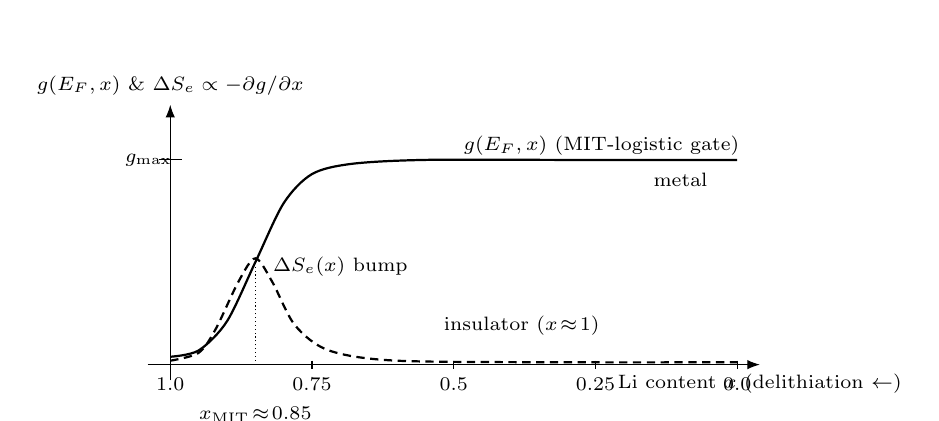
\begin{tikzpicture}[x=7.2cm,y=1.0cm]
% x-axis is Li content x, decreasing to the right (delithiation -> )
\draw[-{Latex[length=1.6mm]}] (-0.04,0) -- (1.04,0) node[below,font=\scriptsize] {Li content $x$ (delithiation $\leftarrow$)};
\draw[-{Latex[length=1.6mm]}] (0,-0.2) -- (0,3.3) node[above,font=\scriptsize] {$g(E_F,x)$ \&\ $\Delta S_e\propto-\partial g/\partial x$};
\foreach \xx/\lab in {0.0/1.0,0.25/0.75,0.5/0.5,0.75/0.25,1.0/0.0} {\draw (\xx,0.05)--(\xx,-0.05) node[below,font=\scriptsize] {\lab};}
\draw (-0.02,2.6)--(0.02,2.6) node[left,font=\scriptsize] {$g_{\max}$};
% g(E_F): logistic gate, ~0 at x=1 (left? no: x=1 is left tick label)
% map: tick at xx=0 -> x=1 (insulator), xx=1 -> x=0 (metal). x_MIT=0.85 -> xx=0.15
% g rises as we go right (x decreasing). center at xx=0.15
\draw[thick] plot[smooth] coordinates {(0.0,0.10) (0.05,0.18) (0.10,0.55) (0.15,1.30) (0.20,2.05) (0.25,2.42) (0.32,2.55) (0.45,2.6) (0.7,2.6) (1.0,2.6)};
\node[right,font=\scriptsize] at (0.5,2.78) {$g(E_F,x)$ (MIT-logistic gate)};
\node[font=\scriptsize] at (0.62,0.5) {insulator ($x\!\approx\!1$)};
\node[font=\scriptsize] at (0.9,2.35) {metal};
% Delta S_e ~ -dg/dx : a localized bump near x_MIT (xx=0.15)
\draw[densely dashed,thick] plot[smooth] coordinates {(0.0,0.05) (0.05,0.15) (0.08,0.45) (0.12,1.05) (0.15,1.35) (0.18,1.05) (0.22,0.50) (0.28,0.18) (0.4,0.05) (0.7,0.03) (1.0,0.03)};
\node[font=\scriptsize] at (0.30,1.25) {$\Delta S_e(x)$ bump};
\draw[densely dotted] (0.15,0)--(0.15,1.35);
\node[below,font=\scriptsize] at (0.15,-0.42) {$x_\mathrm{MIT}\!\approx\!0.85$};
\end{tikzpicture}
\caption{LCO 전자 엔트로피의 MIT-logistic 게이트(신규). 실선 $=g(E_F,x)$(식~\eqref{eq:ggate}): $x\!\approx\!1$
절연체에서 $\approx0$, 탈리튬화로 $x_\mathrm{MIT}\!\approx\!0.85$ 부근에서 metal 의 $g_{\max}\!=\!13$ e/eV 로 켜진다.
파선 $=$ 탈리튬화 시 방출되는 부분몰 전자 엔트로피 $|\Delta S_e|=-\partial S_e/\partial x\propto-\partial g/\partial x>0$
(식~\eqref{eq:dSe}$\cdot$닫힌식~\eqref{eq:dSegate}; 삽입 기준 $\Delta S_e=\partial S_e/\partial x<0$ 의 절댓값으로,
$x_\mathrm{MIT}$ 에서 $\sigma(1-\sigma)$ 가 최대): 천이 중심의 \emph{국소
봉우리}다 — 작지만(O3 부분몰 $\approx0.18\,k_B$/atom) MIT 구간에만 켜지는 게이트라 config 단독으로 대체 불가.
$\Delta S_{e,j}\propto T$ 라 다른 항과 달리 전자 기여의 $\partial U/\partial T$ 가 $T$ 에 선형(\S\ref{sec:lco-Se}; U-이동은
$\propto T^2$). 흑연엔 이 봉우리가 없다($g(E_F)$ 변화 미미).}
\label{fig:lco-electronic}
\end{figure}

이 전자항이 \S\ref{sec:sum} 의 $\Delta S_{\rxn,j}^\mathrm{cat}$ 분해에서 셋째 성분으로 plug-in 되며(흑연은 이 자리가 0),
forward 코드는 전이 파라미터를 LCO 로 갈아 끼우고 이 항 하나를 더하는 것만으로 LCO 에 적용된다(\S\ref{sec:lco-code}).

% ====================================================================
\section{평형 peak — $|I|\to0$ 기준선 (N6)}\label{sec:eqpeak}
% ====================================================================
코드는 평형 점유에서 곧바로 평형 peak 모양 $\xi_\eq(1-\xi_\eq)/w$ 를 만든다. 이것이 전류가 없을 때($|I|\to0$)의
기준선이며, 동역학 꼬리가 무시될 만큼 작을 때 코드가 직접 쓰는 항이다.

\textbf{(a) 출발 — 전하 보존식.} 관측 $\dd Q/\dd V$ 는 전하 보존식 $Q_\cell q=Q_\bg(V_n)+\sum_jQ_j\xi_j$ 를 궤적
$q$ 로 미분해 닫힌다 — 양변을 $q$ 로 미분하면 $Q_\cell=C_\bg\,\dd V_n/\dd q+\sum_jQ_j\,\dd\xi_j/\dd q$ 이고,
$\dd V_n/\dd q$ 로 나누면 $\dd Q/\dd V_n=C_\bg+\sum_jQ_j\,\dd\xi_j/\dd V_n$ 이다. \textbf{(b) 연산 — logistic
미분의 종 항등식.} 평형 추종이면 $\dd\xi_j/\dd V_n$ 에 평형 기울기가 들어가고, $z\equiv\sigma_d(V-U_j^{\,d})/w_j$ 로
$\xi_\eq=(1+e^{-z})^{-1}$ 를 미분하면
\begin{equation}
\frac{\dd\xi_\eq}{\dd z}=\frac{e^{-z}}{(1+e^{-z})^2}
=\underbrace{\frac{1}{1+e^{-z}}}_{\xi_\eq}\cdot\underbrace{\frac{e^{-z}}{1+e^{-z}}}_{1-\xi_\eq}
=\xi_\eq(1-\xi_\eq)
\label{eq:belliden}
\end{equation}
— $\xi(1-\xi)$ 는 $\xi=\tfrac12$ 에서 최대 $\tfrac14$ 인 종이다. \textbf{(c) 중간식 — 연쇄율.} 연쇄율
$\dd z/\dd V=\sigma_d/w_j$ 를 곱하면 $\dd\xi_{\eq,j}/\dd V=\sigma_d\,\xi_\eq(1-\xi_\eq)/w_j$. \textbf{(d) 박스.}
이를 보존식 미분에 넣으면 전이 $j$ 의 평형 peak 이 닫힌다:
\begin{equation}
\frac{\dd\xi_{\eq,j}}{\dd V}=\frac{\sigma_d\,\xi_{\eq,j}(1-\xi_{\eq,j})}{w_j}
\;\Longrightarrow\;
\boxed{\;\Big(\frac{\dd Q}{\dd V}\Big)^\eq_j
=Q_j\,\frac{\xi_{\eq,j}(1-\xi_{\eq,j})}{w_j}
=Q_j\,\Big|\frac{\dd\xi_{\eq,j}}{\dd V}\Big|\;.}
\label{eq:eqpeak}
\end{equation}
이것이 코드의 \code{peak\_shape = ksi\_eq * (1 - ksi\_eq) / w} 이며, 메서드 \code{equilibrium} 이 전이별로 이 항만
합산한 것($C_\bg+\sum_jQ_j\xi_\eq(1-\xi_\eq)/w$)이다. 부호 — $\sigma_d$ 가 미분에서 한 번 들어오지만 peak 모양은
절댓값 $|\dd\xi/\dd V|=\xi_\eq(1-\xi_\eq)/w$ 로 양수이고 방향 불변이다($\xi(1-\xi)\ge0$). 세 양 — 위치 $=$ 중심
$U_j^{\,d}$, 순높이 $=Q_j/(4w_j)$($\xi=\tfrac12$ 에서 $\xi(1-\xi)=\tfrac14$), 배경 차감 면적 $=Q_j$
($\int_0^1\dd\xi=1$, 식~\eqref{eq:belliden} 의 종이 $\dd\xi_\eq$ 의 치환적분이라 면적 $1$) — 가 이 한 식에서 읽힌다.

코드의 사용 조건은 ``지연 길이가 격자에 비해 작을 때''다 — 다음 절이 그 지연 길이 $L_V$ 를 세우고, $L_V$ 가 격자
몇 칸보다 작으면(또는 동역학 키가 없으면) 코드는 식~\eqref{eq:eqpeak} 의 평형 종을 직접 쓴다. 이것이 $|I|\to0$ 환원이다.

\subsection{LCO dQ/dV peak — 양극 영역의 세 봉우리}\label{sec:lco-peak}
평형 peak 식~\eqref{eq:eqpeak} $Q_j\,\xi_\eq(1-\xi_\eq)/w_j$ 는 전극을 가리지 않으므로, LCO 양극에도 그대로 적용된다 —
위치 $=$ 중심 $U_j^{\,d}$, 순높이 $=Q_j/(4w_j)$, 면적 $=Q_j$ 의 세 양이 표~\ref{tab:lco-staging} 의 LCO 전이로 읽힌다.
흑연이 $\sim$0.085--0.21 V 에 네 봉우리를 남기듯, LCO 하프셀은 \emph{양극 전위 영역}에 세 봉우리를 남긴다 — T1 의
$\sim$3.90 V(MIT plateau), T2 의 $\sim$4.05 V, T3 의 $\sim$4.17--4.20 V(T2 와 한 쌍의 좁은 order--disorder 봉우리)다.
폭은 흑연과 같은 $w_j=n_jRT/F$ 이며($\Omega_j>2RT$ 면 좁힘 옵션 식~\eqref{eq:weff}), order--disorder 의 큰 $\Omega$
가 T2$\cdot$T3 를 흑연보다 날카롭게 만든다. T1 의 위치는 \S\ref{sec:lco-electronic} 의 전자항이
$\Delta S_{\rxn,1}^\mathrm{cat}$ 를 통해 $U_1(T)$ 의 \emph{온도 이동}에 기여하므로(식~\eqref{eq:lco-dUdT}), 다온도
dQ/dV 에서 T1 봉우리의 \emph{온도 이동률} $\partial U_1/\partial T$ 가 $T$ 에 선형으로 커지는 것이 전자항의 관측
신호다($\Delta S_{e,1}\propto T$, \S\ref{sec:lco-Se} — 위치 자체가 $T$-선형이 아니라 \emph{이동률}이 $T$-선형, 곧 위치
이동은 $\propto T^2$). 도핑은 \S\ref{sec:lco-hys} 대로 봉우리를 smear$\cdot$shift 시킨다.

% ====================================================================
\section{동역학 지연 길이 $L_V$ (N7)}\label{sec:lag}
% ====================================================================
유한 전류에서는 평형 목표 $\xi_\eq$ 를 점유가 즉시 따라가지 못하고 뒤처진다 — 그 지연이 peak 의 꼬리다. 코드는 전이당
하나의 지연 길이 $L_{V,j}$ 를 resolver \code{\_resolve\_lag\_length} 로 구한다. 이 절은 그 사슬
$\mathcal A\to\chi_d\to\Delta H_a^\eff\to L_q\to L_V$ 를, 운동방정식의 보편형에서 한 단계씩 닫는다.

\subsection{지연의 보편 방정식과 용량축 길이 $L_q$}
\textbf{(a) 출발 — 운동방정식을 용량축으로.} \S\ref{sec:width} 의 운동방정식 $\dd\xi_j/\dd t=k_j(\xi_{\eq,j}-\xi_j)$
을, 정전류에서 성립하는 $\dd q/\dd t=|I|/Q_\cell$ 로 나누면 $\dd\xi_j/\dd q=(Q_\cell k_j/|I|)(\xi_{\eq,j}-\xi_j)$.
\textbf{(b) 연산 — 지연 변수.} 지연 $r_j\equiv\xi_{\eq,j}-\xi_j$ 의 변화율 $\dd r_j/\dd q=\dd\xi_{\eq,j}/\dd q-\dd\xi_j/\dd q$
에 위 식을 넣으면 \textbf{(c) 중간식.}
\begin{equation}
\frac{\dd r_j}{\dd q}=\frac{\dd\xi_{\eq,j}}{\dd q}-\frac{Q_\cell k_j}{|I|}\,r_j,
\label{eq:Lqmid}
\end{equation}
\textbf{(d) 박스 — 용량축 길이 정의.} 계수의 역수가 용량축 지연 길이다:
\begin{equation}
\frac{\dd r_j}{\dd q}=\frac{\dd\xi_{\eq,j}}{\dd q}-\frac{r_j}{L_{q,j}},
\qquad \boxed{\;L_{q,j}=\frac{|I|}{Q_\cell\,k_j}\;.}
\label{eq:Lq}
\end{equation}
$L_{q,j}$ 는 요구($|I|/Q_\cell$)와 공급($k_j$)의 비 그 자체다 — 근본식의 세 인자가 전부 이 한 양을 통해 꼬리로
들어온다. 완화 속도 $k_j$ 는 평형 근방 선형 완화에서 정$\cdot$역 속도의 합이다 — detailed balance~\eqref{eq:db} 로
$r_j^-=r_j^+e^{-\mathcal A_j/RT}$ 이므로
\begin{equation}
k_j=r_j^++r_j^-=r_j^+\big(1+e^{-\mathcal A_j/RT}\big),
\qquad r_j^+\simeq k_0\,e^{-(\Delta G_{a,j}^\eff-\chi_d\mathcal A_j)/RT}\ (k_0=k_BT/h),
\label{eq:kuniv}
\end{equation}
이고, 괄호 인자 $(1+e^{-\mathcal A_j/RT})$ 가 역방향 몫의 전부다($\mathcal A\gtrsim3RT$ 면 $1$ 로 죽는다). 이 두 인자가
아래 $L_q$ 평가식의 분모와 forward 지수를 각각 채운다.

\subsection{컷 affinity $\mathcal A$ — 꼬리 시작점의 구동력}
$L_q$ 는 전이당 한 점(꼬리 컷점 $q_a$)에서 \emph{상수로 동결}된다. \textbf{(a) 출발 — 컷의 정의.} 컷점은 원천
$\dd\xi_\eq/\dd q$ 가 정점의 일정 분율(약 $5\%$)로 떨어지는 좌표이고, \textbf{(b)(c) 연산$\cdot$중간식 — 컷의 구동력.}
그곳의 구동력은 $\mathcal A=z_\mathrm{cut}\cdot n_jRT$ 다($z_\mathrm{cut}=4.357$ 이 그 미분 $\dd\xi_\eq/\dd q$ 의 $5\%$
컷에 대응 — 점유 $\xi_\eq$ 자체가 아니라 미분 기준; logistic 미분 종의 $5\%$ 폭이 중심에서 $\pm z_\mathrm{cut}\,RT/F$
규모라 $\mathcal A=z_\mathrm{cut}n_jRT$). \textbf{(d) 박스 — 상한과 함께.}
\begin{equation}
\mathcal A=\min\!\big(z_\mathrm{cut}\,n_j\,RT,\;A_\mathrm{cap}\,RT\big),
\qquad z_\mathrm{cut}=4.357,\ A_\mathrm{cap}=4.0\ (\text{기본; }z_\mathrm{cut}\text{ 는 미분 }5\%\text{ 컷의 선택값}).
\label{eq:Acut}
\end{equation}
이것이 코드의 \code{A = min(z\_cut * n\_safe * R*T, A\_cap * R*T)} 다. \emph{부호의 핵심} — 컷 affinity 의 \emph{크기}는
충$\cdot$방전 동일($n_j>0$ 라 항상 양수)이고, 방향은 아래 $\chi_d\cdot\Delta H_a^\eff$ 가 받는다. 방향 부호 $\sigma_d$ 를
$\min$ 안에 넣으면 충전에서 음수 상한이 되는 버그가 생기므로, 코드는 $\sigma_d$ 를 크기에서 빼고 방향은 전달 계수로만
주입한다.

\subsection{방향별 전달 계수와 유효 장벽}
\textbf{(a) 출발 — 합-1 제약.} 전이상태가 정$\cdot$역 장벽을 비대칭으로 가르는 분율 $\chi\in[0,1]$ 의 합-1 제약
($\chi+\chi'=1$, 식~\eqref{eq:db} detailed balance 가 강제)에서, \textbf{(b)(c) 방향별 선택.} 방향별 전달 계수는
\begin{equation}
\chi_d=\chi_\mathrm{split}(\chi,\sigma_d)=
\begin{cases}\chi & \sigma_d\ge0\ (\text{방전})\\ 1-\chi & \sigma_d<0\ (\text{충전}).\end{cases}
\label{eq:chid}
\end{equation}
이것이 \code{func\_chi\_d(chi, sigma\_d)} 이며(생성자 \code{chi\_split} 로 다른 규칙 주입 가능). \textbf{(d) 유효 장벽.}
깊은 꼬리에서 방전은 $\xi\to1$, 충전은 $\xi\to0$ 거울이라 역방향 장벽의 상수 몫이 같은 $+\Omega$ 로 흡수된다 — 꼬리
구동력 $\mathcal A_j=sF(V-U_j)-\Omega_j(1-2\xi_j)$ 에서 상호작용 몫 $-\Omega(1-2\xi)$ 가 깊은 꼬리에서 상수 $+\Omega$ 로
가고, 이것이 활성화 엔탈피에 흡수되어 유효값이 된다:
\begin{equation}
\boxed{\;\Delta H_{a,j}^\eff=\Delta H_{a,j}-\chi_d\,\Omega_j\;.}
\label{eq:dHeff}
\end{equation}
이것이 \code{func\_dH\_a\_eff(dH\_a, Omega, chi\_d)} 이고, 코드는 \code{use\_dH\_eff} 가 꺼져 있으면 보강 없이
$\Delta H_a$ 를 그대로 쓴다(헬퍼 \code{\_chi\_and\_dH\_eff} 가 $(\chi_d,\Delta H_a^\eff)$ 를 한 곳에서 낸다).

\subsection{$L_q$ 의 평가와 전압축 환산 $L_V$}
\textbf{(a) 출발 — 정$\cdot$역 합과 Eyring prefactor.} 식~\eqref{eq:kuniv} 의 $k_j=r_j^+(1+e^{-\mathcal A_j/RT})$ 와
$r_j^+\simeq k_0e^{-(\Delta G_a^\eff-\chi_d\mathcal A)/RT}$($k_0=k_BT/h$)을 식~\eqref{eq:Lq} 의 $L_{q,j}=|I|/(Q_\cell k_j)$
에 넣으면 \textbf{(b)(c) 연산$\cdot$중간식 — $\Delta G_a^\eff=\Delta H_a^\eff-T\Delta S_a$ 로 갈라 적기.}
\begin{equation}
L_{q,j}=\frac{|I|}{Q_\cell}\cdot\frac{h}{k_BT}\cdot
\frac{e^{(\Delta H_{a,j}^\eff-T\Delta S_{a,j}-\chi_d\mathcal A)/RT}}{1+e^{-\mathcal A/RT}},
\label{eq:Lqmid2}
\end{equation}
\textbf{(d) 박스 — 특성 온도로 묶기.} 앞 인자를 $T_*\equiv|I|h/(Q_\cell k_B)$ 로 묶고 forward 지수를 분리하면
\begin{equation}
L_{q,j}=\frac{T_*}{T}\,\frac{\exp\!\big[(\Delta H_{a,j}^\eff-T\Delta S_{a,j})/RT\big]}{1+e^{-\mathcal A/RT}}
\,e^{-\chi_d\mathcal A/RT},
\qquad T_*\equiv\frac{|I|\,h}{Q_\cell\,k_B}.
\label{eq:Lqfull}
\end{equation}
\code{func\_L\_q(T, I, Q\_cell, dH\_a, dS\_a, x, A)} 가 이 로그를
\code{ln\_Lq = ln(T\_attempt/T) - ln(1+e\^{-A/RT}) + dG\_a/RT - x*A/RT} 로 적고($T_\mathrm{attempt}=(I/Q_\cell)h/k_B=T_*$,
$x=\chi_d$, $\dd G_a=\Delta H_a^\eff-T\Delta S_a$) 지수화한다. \emph{암묵 전제 명시} — 식~\eqref{eq:Lqfull} 의
$\Delta H_a^\eff$ 는 \code{func\_L\_q} 의 \code{dH\_a} 인자로 들어가는 값 \code{dH\_a\_use} 이고, 이것은
\code{use\_dH\_eff=True} 일 때만 식~\eqref{eq:dHeff} 의 $\Delta H_a-\chi_d\Omega$ 와 같다 — 꺼져 있으면 그대로
$\Delta H_a$ 다(\code{\_chi\_and\_dH\_eff} 의 분기). 전압축으로 옮기면, 컷점 OCV 기울기를 곱한다 — 꼬리 진폭이
용량축 $1/L_q$ 와 분모 $\dd V_n/\dd q$ 가 묶여 전압축 길이로 정리되는 것이다:
\begin{equation}
\boxed{\;L_{V,j}=\Big|\frac{\dd V}{\dd q}\Big|_{q_a}\,L_{q,j}\;=\;|\code{dVdq\_qa}|\cdot L_{q,j}\;.}
\label{eq:LV}
\end{equation}
코드의 \code{return abs(dVdq\_qa) * L\_q} 다. \emph{부호의 핵심} — 컷 affinity $\mathcal A$ 가 전이당 컷 상수라
($\S\ref{sec:lag}$ 의 동결), 코드 안에서 $L_q$ 는 $V$ 의 함수로 다시 미분되지 않는다: \emph{운영상 실현 미분은}
$\partial\ln L_q/\partial V=0$ 이다(전이당 한 스칼라). 부등식 $\partial\ln L_q/\partial V<0$ 은 \emph{물리적 동기}로 읽어야
한다 — 만일 $\mathcal A$ 를 컷에 동결하지 않고 국소 구동력 $\mathcal A=\sigma_dF(V_n-U)$ 로 두면 $V\!\uparrow\Rightarrow
\mathcal A\!\uparrow\Rightarrow$ 유효 장벽$\downarrow\Rightarrow L_q\downarrow$(꼬리 짧아짐)이고, 이 단조성이 ``꼬리 컷점을
원천 정점의 일정 분율로 잡는다''는 컷 규칙의 정당성이다. 곧 부등식은 컷점 선택의 근거이지 코드가 격자마다 평가하는 양이
아니다. 한편 $|I|$ 의존은 동결 뒤에도 살아 있다 — $L_q\propto|I|$($T_*\propto|I|$)라 $|I|\to0$
에서 $L_V\to0$, 다음 절의 꼬리가 사라지고 평형 peak 으로 환원된다. 직접 지정 \code{'L\_V'} 가 있으면 동역학을 우회해
그 값을 쓰고, $I\le0$ 이거나 \code{dH\_a} 키가 없으면 $L_V=0$ 이다.

\begin{codebox}
\textbf{N7 진행.} \code{n\_safe=|n\_j|} $\to$ $\mathcal A$(식~\eqref{eq:Acut}) $\to$
\code{(chi\_d, dH\_a\_use)=\_chi\_and\_dH\_eff(...)} (식~\eqref{eq:chid}$\cdot$\eqref{eq:dHeff}) $\to$
\code{L\_q=func\_L\_q(...,x=chi\_d,A=A)} (식~\eqref{eq:Lqfull}) $\to$ \code{L\_V=|dVdq\_qa|*L\_q} (식~\eqref{eq:LV}).
전이당 \emph{상수}(대표 $T_\rep\cdot$대표 $n$)로 한 번 평가한다.
\end{codebox}

% ====================================================================
\section{인과 기억 꼬리와 충전 격자 역전 (N8)}\label{sec:tail}
% ====================================================================
지연 길이 $L_{V,j}$ 가 충분히 크면($\ge$ 격자 몇 칸) 코드는 평형 종 대신 \emph{인과 기억 꼬리}를 만든다. 이 절이 그
합성곱과, ★충전에서의 격자 역전을 닫는다 — 본 문건의 가장 미묘한 부호 자리다.

\subsection{지수 기억 — 일반해의 이산형}
\textbf{(a) 출발 — 1계 선형 ODE.} 지연 방정식~\eqref{eq:Lq} 는 1계 선형이라 적분인자 $e^{q/L_{q,j}}$ 로 닫힌 해를 갖는다.
\textbf{(b) 연산 — 적분인자.} 양변에 $e^{q/L_{q,j}}$ 를 곱하면 좌변이 완전 미분으로 묶이고
\begin{equation}
\frac{\dd}{\dd q}\Big(r_j\,e^{q/L_{q,j}}\Big)
=e^{q/L_{q,j}}\Big(\frac{\dd r_j}{\dd q}+\frac{r_j}{L_{q,j}}\Big)
=e^{q/L_{q,j}}\,\frac{\dd\xi_{\eq,j}}{\dd q},
\label{eq:intfactor}
\end{equation}
\textbf{(c) 중간식 — 적분해 일반해.} $q_0$ 부터 적분하고 $e^{-q/L_{q,j}}$ 를 곱해 $r_j$ 를 꺼내면
\begin{equation}
r_j(q)=r_j(q_0)\,e^{-(q-q_0)/L_{q,j}}
+\int_{q_0}^{q}e^{-(q-q')/L_{q,j}}\,\frac{\dd\xi_{\eq,j}}{\dd q'}\,\dd q'
\label{eq:memory}
\end{equation}
— 초기 지연의 지수 감쇠 $+$ 과거 목표 변화율을 지수 커널 $K(\Delta q)=e^{-\Delta q/L_q}$ 로 가중한 \emph{기억}의
합성곱이다(계는 길이 $L_q$ 만큼의 최근 과거만 기억). \textbf{(d) 박스 — 이산 저역통과.} 이산 격자에서 이 1차 저역통과는
한 칸당 감쇠 $\rho=\exp(-\Delta_\mathrm{grid}/L_V)$ 의 점화식이다(연속해~\eqref{eq:memory} 를 격자 간격 $\Delta_\mathrm{grid}$
로 이산화하면 한 칸 전파가 $e^{-\Delta_\mathrm{grid}/L_V}$ 가중):
\begin{equation}
\xi_{\mathrm{lag},i}=\rho\,\xi_{\mathrm{lag},i-1}+(1-\rho)\,\xi_{\eq,i}
\label{eq:lowpass}
\end{equation}
이고, 코드 \code{\_causal\_lowpass} 가 이를 (가능하면) \code{scipy.signal.lfilter} 의 계수
$[1-\rho]/[1,-\rho]$ 로, 아니면 같은 점화식 루프로 평가한다. $L_V\le0$ 이거나 비유한이면 원신호를 그대로 돌린다.
그림~\ref{fig:relaxode} 가 목표 $\xi_\eq$ 와 뒤처진 $\xi_\mathrm{lag}$, 그 차 $r=\xi_\eq-\xi_\mathrm{lag}$ 를 보인다.

\begin{figure}[t]
\centering
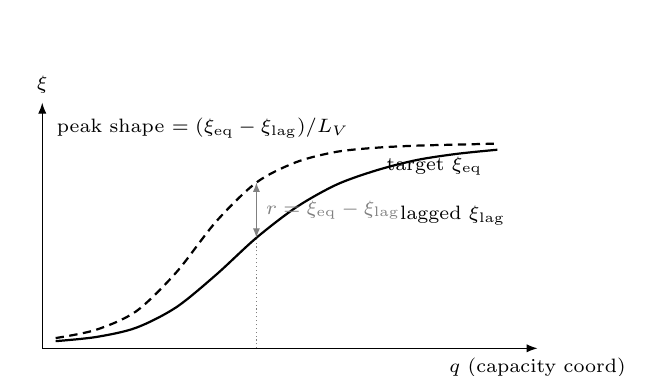
\begin{tikzpicture}[x=1.7cm,y=1.3cm]
% relaxation ODE: target xi_eq (step-like rise) and lagged response
\draw[-{Latex[length=1.4mm]}] (-0.1,0) -- (3.6,0) node[below,font=\scriptsize] {$q$ (capacity coord)};
\draw[-{Latex[length=1.4mm]}] (-0.1,0) -- (-0.1,2.4) node[above,font=\scriptsize] {$\xi$};
% target xi_eq: smooth rising sigmoid to 2
\draw[densely dashed,thick] plot[smooth] coordinates {(0,0.10) (0.3,0.18) (0.6,0.36) (0.9,0.74) (1.2,1.24) (1.5,1.62) (1.8,1.82) (2.1,1.92) (2.4,1.96) (2.7,1.98) (3.0,1.99) (3.3,2.0)};
\node[right,font=\scriptsize] at (2.4,1.78) {target $\xi_\eq$};
% lagged xi (follows behind, smaller, shifted right)
\draw[thick] plot[smooth] coordinates {(0,0.07) (0.3,0.11) (0.6,0.20) (0.9,0.40) (1.2,0.72) (1.5,1.08) (1.8,1.38) (2.1,1.60) (2.4,1.74) (2.7,1.84) (3.0,1.90) (3.3,1.94)};
\node[right,font=\scriptsize] at (2.5,1.30) {lagged $\xi_\mathrm{lag}$};
% gap arrow r = xi_eq - xi_lag at q=1.5
\draw[{Latex[length=1.2mm]}-{Latex[length=1.2mm]},gray] (1.5,1.08) -- (1.5,1.62) node[pos=0.5,right,font=\scriptsize] {$r=\xi_\eq-\xi_\mathrm{lag}$};
\draw[densely dotted,gray] (1.5,0) -- (1.5,1.08);
\node[font=\scriptsize] at (1.1,2.15) {peak shape $=(\xi_\eq-\xi_\mathrm{lag})/L_V$};
\end{tikzpicture}
\caption{지연 ODE 의 완화(신규). 파선 $=$ 평형 목표 $\xi_\eq(q)$, 실선 $=$ 점화식~\eqref{eq:lowpass} 으로 뒤처진
$\xi_\mathrm{lag}$. 둘의 차 $r=\xi_\eq-\xi_\mathrm{lag}$ 가 지연이고, peak 모양 $(\xi_\eq-\xi_\mathrm{lag})/L_V$
(식~\eqref{eq:peakshape})는 이 차를 길이로 나눈 이산 미분이다. 이 매끈한 차분이 미분 $\dd\xi_\eq/\dd V$ 로 수렴하는
극한은 오히려 $L_V\gg\Delta_\mathrm{grid}$($\rho\to1$, 커널이 진짜 미분이 되는 쪽)이다 — 그림은 그 영역을 그린다.
반대로 $L_V$ 가 작아지는 평형 회복은 이 매끈한 차분의 극한이 아니라 코드의 분기 스위치(식~\eqref{eq:branch})가
담당해 평형 종(식~\eqref{eq:eqpeak})으로 직접 떨어뜨린다(문턱 진폭 불연속·자세한 논증은 본문 \S\ref{sec:tail}).}
\label{fig:relaxode}
\end{figure}

\subsection{peak 모양 — 평형에서 지연을 뺀 것}
\textbf{(a)(b)(c) 출발$\cdot$연산$\cdot$중간식.} 진행률은 어디서나 $\xi_j=\xi_{\eq,j}-r_j$ 이고(지연 $r_j$ 는
일반해~\eqref{eq:memory} 가 전 구간 결정), 그 미분 $\dd\xi_j/\dd V=\dd\xi_{\eq,j}/\dd V-\dd r_j/\dd V$ 를 보존식
$\dd Q/\dd V=C_\bg+\sum Q_j\,\dd\xi_j/\dd V$ 에 넣은 ``평형 전환율에서 지연을 뺀 것''이다. 이산 격자에서 이 차분은
$(\xi_\eq-\xi_\mathrm{lag})$ 를 길이로 나눈 형태가 된다. \textbf{(d) 박스.}
\begin{equation}
\boxed{\;\text{peak\_shape}=\frac{\xi_{\eq}-\xi_{\mathrm{lag}}}{L_{V,j}}\;.}
\label{eq:peakshape}
\end{equation}
이것이 코드의 \code{peak\_shape = (ksi\_eq - occ\_lagged) / lag\_len\_V} 다($\xi_\mathrm{lag}$ 는 점화식~\eqref{eq:lowpass}
의 출력). 이 차분이 매끈한 미분 $\dd\xi_\eq/\dd V$ 로 수렴하는 극한은 $L_V\gg\Delta_\mathrm{grid}$ 쪽이다 —
이때 한 칸 감쇠 $\rho=e^{-\Delta_\mathrm{grid}/L_V}\to1$ 이라 점화식~\eqref{eq:lowpass} 의 커널이 길이 $L_V$ 의 진짜 1차
저역통과(미분 커널)로 살아나, $(\xi_\eq-\xi_\mathrm{lag})/L_V$ 가 평형 종에 꼬리를 더한 모양을 낸다. \emph{반대로}
$L_V$ 가 작아지는 평형 회복은 이 차분의 극한이 \emph{아니다}: $L_V\to0$ 이면 $\rho\to0$ 이라 $\xi_\mathrm{lag}\to\xi_\eq$
(같은 칸 — 한 칸 지연이 아니다), 곧 분자 $(\xi_\eq-\xi_\mathrm{lag})\to0$ 과 분모 $L_V\to0$ 이 함께 사라지는 $0/0$ 이라
식~\eqref{eq:peakshape} 가 종으로 매끈히 환원되지 않는다. 그 작은 $L_V$ 환원은 코드의 분기 스위치가 담당한다 —
$L_V<\nu\,\Delta_\mathrm{grid}$ 면 식~\eqref{eq:peakshape} 를 평가하지 않고 평형 종 식~\eqref{eq:eqpeak} 을 직접 쓴다:
\begin{equation}
\text{peak\_shape}=
\begin{cases}
\xi_\eq(1-\xi_\eq)/w & L_{V,j}<\nu\,\Delta_\mathrm{grid}\ \text{(또는 비유한)}\quad[\text{평형, 식~\eqref{eq:eqpeak}}]\\[2pt]
(\xi_\eq-\xi_\mathrm{lag})/L_{V,j} & \text{그 외}\quad[\text{꼬리, 식~\eqref{eq:peakshape}}],
\end{cases}
\label{eq:branch}
\end{equation}
$\nu=\code{min\_lag\_grid\_steps}=2$ 다(지연이 격자 두 칸보다 짧으면 평형 종 직접). 이 전환은 \emph{매끈한 handoff 가 아니라
이산 모드 스위치}임에 주의한다 — 문턱 $L_V=\nu\Delta_\mathrm{grid}$ 에서 꼬리 분기의 진폭과 평형 종의 진폭
($\propto 1/w$)이 정확히 같게 맞춰져 있지 않아 작은 불연속이 생길 수 있다. 이는 sub-grid 지연의 수치 불안정을 피하기
위한 실용적 선택이며($\nu$ 를 키우면 전환점이 더 깊은 꼬리로 밀려 점프가 작아진다), 꼬리식 자신의 $L_V\to0$ 소멸
($0/0$)은 이미 평형 분기 영역에 들어가 코드가 꼬리식으로 평가하지 않는 구간이다.

\subsection{★충전 격자 역전 — 인과 방향}
인과 합성곱~\eqref{eq:memory} 은 ``진행 방향의 과거''를 기억한다. 방전($\sigma_d=+1$)은 진행이 $V$ 증가 방향이라 격자
오름차순이 곧 시간 순서이고, 저역통과를 격자 그대로 적용한다. 충전($\sigma_d=-1$)은 진행이 $V$ 감소 방향 — 격자
오름차순의 \emph{역}이 시간 순서다. 따라서 충전은 격자를 뒤집어 필터하고 되돌린다:
\begin{equation}
\xi_\mathrm{lag}=
\begin{cases}
\code{causal\_lowpass}(\xi_\eq) & \sigma_d\ge0\ (\text{방전})\\[2pt]
\code{causal\_lowpass}(\xi_\eq[::-1])[::-1] & \sigma_d<0\ (\text{충전}).
\end{cases}
\label{eq:reversal}
\end{equation}
이것이 코드의 \code{occ\_lagged = lowpass(ksi\_arr[::-1])[::-1]} (충전 분기)다. 이 역전이 없으면 충전 꼬리가
\emph{미래}를 기억하는 비인과 신호가 되어 peak 가 엉뚱한 쪽으로 번진다. \emph{부호 결과} — 충전 $\dd Q/\dd V$ 는 방전의
거울상이고, peak\_shape $=(\xi_\eq-\xi_\mathrm{lag})/L_V$ 는 양수를 유지한다(꼬리가 진행 방향 뒤쪽, 곧 충전에서는
$V$ 가 큰 쪽으로 늘어진다). 그림~\ref{fig:reversal} 가 두 방향을 나란히 보인다.

\begin{figure}[t]
\centering
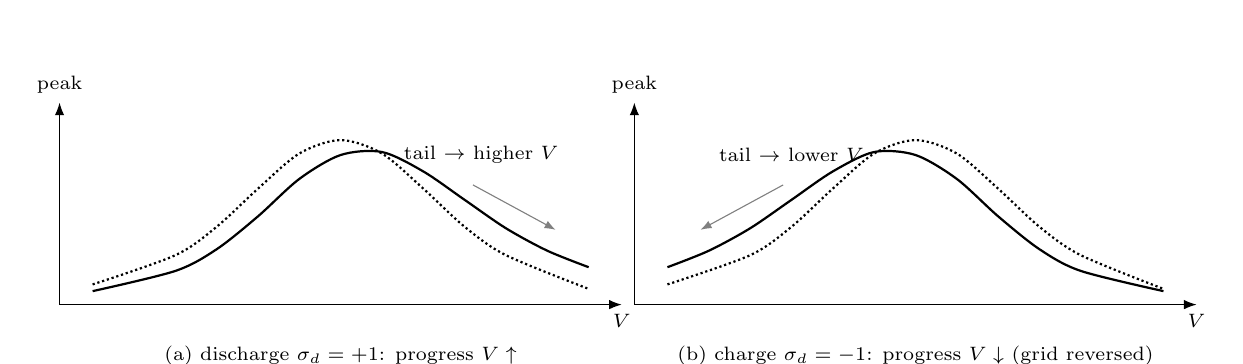
\begin{tikzpicture}[x=1.05cm,y=0.95cm]
% discharge panel (left)
\begin{scope}
\draw[-{Latex[length=1.6mm]}] (-3.4,0) -- (3.4,0) node[below,font=\scriptsize] {$V$};
\draw[-{Latex[length=1.6mm]}] (-3.4,0) -- (-3.4,2.7) node[above,font=\scriptsize] {peak};
% bell (equilibrium) dotted
\draw[densely dotted,thick] plot[smooth] coordinates {(-3,0.27) (-2,0.66) (-1.5,1.04) (-1,1.55) (-0.5,2.02) (0,2.2) (0.5,2.02) (1,1.55) (1.5,1.04) (2,0.66) (3,0.21)};
% discharge tail: shifted/broadened to higher V (right)
\draw[thick] plot[smooth] coordinates {(-3,0.18) (-2,0.45) (-1.5,0.74) (-1,1.18) (-0.5,1.68) (0,2.0) (0.5,2.04) (1,1.78) (1.5,1.4) (2,1.02) (2.5,0.72) (3,0.5)};
\draw[-{Latex[length=1.4mm]},gray] (1.6,1.6)--(2.6,1.0);
\node[font=\scriptsize] at (1.7,2.0) {tail $\to$ higher $V$};
\node[font=\scriptsize,below] at (0,-0.42) {(a) discharge $\sigma_d=+1$: progress $V\uparrow$};
\end{scope}
% charge panel (right)
\begin{scope}[xshift=7.3cm]
\draw[-{Latex[length=1.6mm]}] (-3.4,0) -- (3.4,0) node[below,font=\scriptsize] {$V$};
\draw[-{Latex[length=1.6mm]}] (-3.4,0) -- (-3.4,2.7) node[above,font=\scriptsize] {peak};
\draw[densely dotted,thick] plot[smooth] coordinates {(-3,0.27) (-2,0.66) (-1.5,1.04) (-1,1.55) (-0.5,2.02) (0,2.2) (0.5,2.02) (1,1.55) (1.5,1.04) (2,0.66) (3,0.21)};
% charge tail: mirror — broadened to lower V (left)
\draw[thick] plot[smooth] coordinates {(-3,0.5) (-2.5,0.72) (-2,1.02) (-1.5,1.4) (-1,1.78) (-0.5,2.04) (0,2.0) (0.5,1.68) (1,1.18) (1.5,0.74) (2,0.45) (3,0.18)};
\draw[-{Latex[length=1.4mm]},gray] (-1.6,1.6)--(-2.6,1.0);
\node[font=\scriptsize] at (-1.5,2.0) {tail $\to$ lower $V$};
\node[font=\scriptsize,below] at (0,-0.42) {(b) charge $\sigma_d=-1$: progress $V\downarrow$ (grid reversed)};
\end{scope}
\end{tikzpicture}
\caption{인과 꼬리의 방향(v7-11 유래). 점선 $=$ 평형 종($\xi_\eq(1-\xi_\eq)/w$, 방향 불변). 실선 $=$ peak\_shape
with tail. (a) 방전은 진행이 $V\!\uparrow$ 라 꼬리가 높은 $V$ 쪽으로 늘어진다(격자 그대로). (b) 충전은 진행이
$V\!\downarrow$ 라 격자를 뒤집어 필터($\xi[::-1]\cdots[::-1]$)해 꼬리가 낮은 $V$ 쪽으로 — 방전의 거울. 두 경우 모두
peak 는 양수.}
\label{fig:reversal}
\end{figure}

% ====================================================================
\section{합산과 역보간 (N9)}\label{sec:sum}
% ====================================================================
전이 루프가 각 전이의 peak\_shape 를 (식~\eqref{eq:branch} 의 두 분기로) 만들면, 코드는 용량 가중을 곱해 작업 격자 위
누적에 더하고, 모든 전이가 끝나면 내부 전위 격자로 역보간한다. 보존식 $Q_\cell q=Q_\bg+\sum_jQ_j\xi_j$ 가
$\sum_jQ_j\xi_j$ 꼴이라 관측 ICA 는 배경과 전이별 기여의 선형 합이다 — 합산 자체는 보존식의 직접 미분이라 가정이
아니다(서로소 자리 분해가 전제):
\begin{equation}
\boxed{\;\frac{\dd Q}{\dd V}(V_n)\;=\;C_\bg\;+\;\sum_{j=1}^{N_p}Q_j\,
\big[\text{peak\_shape}_j\big]
\;=\;C_\bg+\sum_jQ_j\big[\text{평형 peak}-\text{지연 꼬리}\big]\;.}
\label{eq:sum}
\end{equation}
코드는 \code{dqdv\_work += tr['Q'] * peak\_shape} 로 누적하고(배경은 루프 전에 깔림), 마지막에
\code{np.interp(V\_n, V\_work, dqdv\_work)} 로 작업 격자에서 내부 전위 격자로 되돌린다(\code{dqdv\_out}).
스칼라 입력이면 첫 성분만 반환한다.

\subsection{staging 전이 초기값 — 피팅 출발점}
4건의 전이 초기값이 \code{GRAPHITE\_STAGING\_LIT} 에 박혀 있다(신뢰값 아닌 \emph{초기값} — 사용자 피팅이 override
전제). 표~\ref{tab:staging} 가 각 인자의 의미와 출발값이다 — 이 표가 있어 ``이 문건만으로 곡선 재현 코드를 짤 수 있다''.

\begin{table}[t]
\centering
\renewcommand{\arraystretch}{1.25}
\caption{전이 초기값 \code{GRAPHITE\_STAGING\_LIT}(4건) — 출발점, 피팅으로 override. $U$ 는 \code{'U'}
폴백이자 $(\Delta H_\rxn,\Delta S_\rxn)$ 정합 목표.}
\label{tab:staging}
\begin{tabular}{l c c c c c c c}
\toprule
stage & $U$ [V] & $\Delta H_\rxn$ & $\Delta S_\rxn$ & $Q$ & $\Omega$ & $\Delta H_a$ & $|\dd V/\dd q|_{q_a}$ \\
 &  & [J/mol] & [J/(mol\,K)] & [$Q_\cell$] & [J/mol] & [J/mol] & [V] \\
\midrule
$4\!\to\!3$   & 0.210 & $-11700$ & $+29.0$ & 0.10 & 6000  & 48000 & 0.30 \\
$3\!\to\!2\mathrm L$ & 0.140 & $-13500$ & $0.0$   & 0.12 & 8000  & 46000 & 0.30 \\
$2\mathrm L\!\to\!2$ & 0.120 & $-13100$ & $-5.0$  & 0.25 & 10000 & 44000 & 0.30 \\
$2\!\to\!1$   & 0.085 & $-13000$ & $-16.0$ & 0.50 & 13000 & 40000 & 0.30 \\
\bottomrule
\end{tabular}
\end{table}

각 전이는 폭 $w$ 폴백(0.020/0.016/0.014/0.012 V)과 $n=1$, $\Delta S_a=0$ 을 함께 갖는다. $\Delta H_\rxn/\Delta S_\rxn$
은 $U(298)$ 정합으로 정해졌고($U=(-\Delta H_\rxn+298.15\Delta S_\rxn)/F$ 가 표의 $U$ 와 일치), $\Delta H_a$ 는 저SOC$\to$
만충에서 감소하는 DFT 활성화 경향, $|\dd V/\dd q|_{q_a}$ 는 컷 OCV 기울기(피팅), $\Omega$ 는 정규용액 추정이다.

\subsection{LCO $\Delta S_{\rxn,j}^\mathrm{cat}$ 분해 — config + vib + electronic}\label{sec:lco-decomp}
흑연에서 합산식~\eqref{eq:sum} 에 들어가는 $\Delta S_{\rxn,j}$ 는 평형 중심 $U_j(T)$ 를 통해 한 덩이로 작용했다. LCO
양극에서는 이 한 덩이가 세 물리 성분의 합임을 명시한다 — 식과 코드 경로는 그대로이고($U_j(T)$ 에 들어가는 $\Delta S$ 의
\emph{내부 분해}만 더한다):
\begin{equation}
\boxed{\;\Delta S_{\rxn,j}^\mathrm{cat}(x,T)=\underbrace{\Delta S_j^\mathrm{config}}_{\text{logistic }w=RT/F\text{ 가 담음}}
+\underbrace{\Delta S_j^\mathrm{vib}}_{\text{음의 baseline}}
+\underbrace{\Delta S_{e,j}^{\,\mathrm{mol}}(x,T)}_{\text{MIT 게이트, 삽입 기준 }<0,\ \propto T\ (\text{몰당 식~\eqref{eq:dSemolar}})}\;.}
\label{eq:lco-decomp}
\end{equation}
세 몫의 역할과 \emph{이중계산 방지}는 다음과 같다.
\begin{itemize}[leftmargin=1.4em,itemsep=2pt]
\item \textbf{config.} O3 영역에서 LCO $\Delta S$ 를 지배($>\tfrac12$\cite{reynier2004}, tier A)하며, 기존 Ch1 logistic 이 이를
\emph{자동 생성}한다 — 봉우리 중심의 표준값 $\Delta S_j^0$ 에 봉우리 내부 항 $R\ln[(1-\xi)/\xi]$ 가 격자기체
점유 분포(\S\ref{sec:dist})에서 따라 나온다. \textbf{★이중계산 금지(B).} 따라서 식~\eqref{eq:lco-decomp} 의
$\Delta S_j^\mathrm{config}$ 자리에는 봉우리 \emph{중심 표준값} $\Delta S_j^0$ 만 넣는다 — 봉우리 내부 조성 의존은
logistic 이 이미 담고 있어 두 번 더하면 안 된다(표~\ref{tab:lco-staging} 의 config 값 = 중심 표준값으로 읽음).
\textbf{★가법성 정당화(T1 MIT, 직교 자유도).} 두 가지를 구분해 못박는다. \emph{(가) 가산성} — config(리튬 자리
\emph{점유 배열}의 자유도)와 $\Delta S_{e,j}$(전도 전자 \emph{밴드 점유}의 자유도)는 서로 다른 자유도라 통계역학적으로
\emph{근사적으로 직교}한다: 두 부분계가 독립인 극한에서 전체 분배함수가 $Z=Z_\mathrm{config}\!\cdot\!Z_\mathrm{elec}$ 로
인수분해되어 $S=S_\mathrm{config}+S_\mathrm{elec}$ 가 교차항(잔차) $0$ 으로 가산된다(MIT 부근에서 리튬 정렬과 전자
밴드채움이 다소 결합하나, 이 결합 몫은 아래 (나)의 슬롯 분리로 따로 통제하므로 분해 자체의 가산성은 선도 차수에서
성립한다). 따라서 식~\eqref{eq:lco-decomp} 의 config$+$elec 를 단순히 더하는 것 자체는 (근사) 직교성으로 정당화된다. \emph{(나) 무이중계산} — 두 항의 합이 측정
$\Delta S$ 를 \emph{초과하지 않음}은 직교성이 아니라 위 ★이중계산 금지(B) 규칙이 보장한다: config 슬롯에 봉우리
\emph{중심값}만, elec 슬롯에 MIT 게이트 \emph{골}만 넣어 각 항이 자기 자유도의 몫만 채우므로, 같은 엔트로피를 두 번
세지 않는다. 곧 직교성은 ``더해도 되는가''(가산성)를, 이중계산 금지 규칙은 ``과대 계상 없는가''(무초과)를 각각 보장한다.
\item \textbf{vib.} 고-$x$ 의 phonon 음의 baseline 으로, Ch1 흑연과 동형이다(흑연 표~\ref{tab:staging} 의 음의
$\Delta S_\rxn$ 에 대응). 별도 식 변화 없음.
\item \textbf{electronic.} \S\ref{sec:lco-electronic} 의 신규 항 $\Delta S_{e,j}(x,T)<0$(닫힌식~\eqref{eq:dSegate},
몰당 환산 식~\eqref{eq:dSemolar} 로 $\Delta S_{e,j}^{\,\mathrm{mol}}=N_A\Delta S_{e,j}$ 가 이 자리에 들어감; \emph{삽입
기준} — $\Delta S_{\rxn,j}$ 슬롯과 일관, 부호 뒤집기 없음; 탈리튬화 시 $|\Delta S_{e,j}|\approx0.18\,k_B$/atom 방출).
흑연엔 0, LCO 는 T1 의 MIT 게이트에서만 켜진다. 셋 중 유일하게 $\propto T$ 라, 다온도 피팅에서 다른 둘과 분리 식별된다.
\end{itemize}
이 세 몫의 합이 식~\eqref{eq:lco-dUdT} 의 $\partial U_j/\partial T=\Delta S_{\rxn,j}^\mathrm{cat}/F$ 를 통해 LCO
$U_j(T)$ 의 온도 이동을 정하고, 그 $U_j(T)$ 가 흑연과 \emph{같은} 합산식~\eqref{eq:sum} 으로 dQ/dV 에 들어간다.
연속 $\Delta S(x)$$\cdot$$g(E_F)(x)$$\cdot$도핑 shift 의 정밀값은 1차 문헌에 없으므로(갭 G1$\cdot$G2$\cdot$G4),
표~\ref{tab:lco-staging}$\cdot$식~\eqref{eq:ggate} 의 초기값을 우리 코인 하프셀 데이터로 round-trip 피팅해 식별한다
— 흑연 ``문헌 초기값 + 데이터 피팅'' 철학 그대로이며, 허위 정밀을 피해 tier 를 병기한다.

\subsection{forward 코드의 LCO 일반화 — 파라미터 교체 + 전자항 plug-in (H)}\label{sec:lco-code}
이 통합의 실용적 결론은 ``같은 코드가 LCO 를 그린다''이다. 그 근거는 \emph{MSMR 동형}이다 — multiphase species
reaction(MSMR) 모델\cite{msmr2024}은 양극 전위를 전이별 logistic 의 합으로 적는다:
\begin{equation}
x_j=\frac{X_j}{1+\exp[\,f(U-U_j^0)/\omega_j\,]},
\label{eq:msmr}
\end{equation}
식~\eqref{eq:msmr} 는 Ch1 의 transition-logistic 식~\eqref{eq:xieq}($\xi_{\eq,j}=1/(1+\exp[-\sigma_d(V-U_j^{\,d})/w_j])$)와
\emph{구조가 동형}이다 — 용량 가중 $X_j\!\leftrightarrow\!Q_j$, 중심 $U_j^0\!\leftrightarrow\!U_j^{\,d}$, 폭 $\omega_j\!\leftrightarrow\!w_j$,
그리고 지수의 \emph{방향 인자} $f\!\leftrightarrow\!-\sigma_d$ 가 1:1 대응한다. 이 방향 인자 대응을 한 번 못박는다. MSMR 의
$f$ 는 종별 부호 인자 $\pm1$ 이고, 식~\eqref{eq:msmr} 의 지수는 $+f(U-U_j^0)$ 인 반면 식~\eqref{eq:xieq} 의 지수는
$-\sigma_d(V-U_j^{\,d})$ 이다. 두 지수가 같은 자리를 채우므로 부호 비교에서 $f=-\sigma_d$ 가 되고, 이로써 탈리튬화/
리튬화 진행 방향이 두 모델에서 일관되게 맞춰진다. 따라서 Ch1 의 곡선 클래스(\code{func\_ksi\_eq}$\cdot$\code{func\_U\_j}$\cdot$합산~\eqref{eq:sum})는
\emph{구조 변경 0}으로 LCO 에 적용되며, 바뀌는 것은 단 둘이다:
\begin{enumerate}[label=(\roman*),leftmargin=2.2em,itemsep=1pt]
\item \textbf{전이 파라미터 교체} — \code{GRAPHITE\_STAGING\_LIT} $\to$ \code{LCO\_STAGING\_LIT}(표~\ref{tab:lco-staging}):
$(\Delta H_\rxn,\Delta S_\rxn,Q,\Omega,\Delta H_a,\dots)$ 값을 양극 영역으로. 코드의 전이 dict 키 구조는 동일하다.
\item \textbf{전자 엔트로피 항 plug-in} — T1 전이의 $\Delta S_{\rxn}$ 평가에 \emph{몰당} 식~\eqref{eq:dSemolar} 의
$\Delta S_{e,j}^{\,\mathrm{mol}}(x,T)=N_A\,\partial S_e/\partial x$ 를 더하는 한 줄(식~\eqref{eq:lco-decomp}). \textbf{★단위 주의} —
forward 슬롯 $\Delta S_{\rxn,j}$ 는 J/(mol\,K) 라, 자리당 식~\eqref{eq:dSe}(차원 $k_B^2$)가 아니라 \emph{$N_A$ 를 곱한}
몰당 식~\eqref{eq:dSemolar} 를 넣어야 한다($N_A$ 배 누락 시 전자항이 $\sim10^{23}$ 배 과소). $g(E_F,x)$ 는
식~\eqref{eq:ggate} 의 게이트로, 초기값 3개를 피팅 인자로 노출.
\end{enumerate}
$\partial U_j/\partial T\leftarrow\Delta S_{\rxn,j}^\mathrm{cat}/F$ 의 경로(식~\eqref{eq:lco-dUdT})는 흑연과 동일하다 —
곧 ``파라미터 +1 항'' 외에 구조 변경이 없다. 이것이 ``흑연 forward 교과서가 LCO 양극까지 한 틀로 닫힌다''의 코드 측
증거이며, 본 챕터가 두 전극을 한 프레임으로 통합한 까닭이다.

\subsection{전체 입력 인자와 기본값 — 피팅 준비}
사용자 목표는 이 모든 인자를 입력으로 노출해 측정 데이터에 Optuna 로 피팅하는 것이다. 곡선식의 모든 기호가 생성자 인자
또는 전이 dict 키이며, 내부 하드코딩 상수는 없다(전부 기본값$+$override). 표~\ref{tab:inputs} 가 전 조정 인자와
기본값이다 — 어느 것을 고정하고 어느 것을 피팅할지는 사용자가 데이터로 정한다(본 문건은 스코프를 정하지 않는다).

\begin{table}[t]
\centering\footnotesize
\renewcommand{\arraystretch}{1.18}
\caption{전체 입력 인자(코드 식별자)와 기본값. 전이 dict 키는 전이별, 생성자 인자는 모델 공통이며 일부는 전이 dict 로
per-transition override 된다($z_\mathrm{cut}$,$A_\mathrm{cap}$,\code{use\_w\_eff},\code{use\_dH\_eff}).}
\label{tab:inputs}
\begin{tabular}{l l l l}
\toprule
인자(코드) & 자리 & 기본값 & 곡선 내 역할(식) \\
\midrule
\multicolumn{4}{l}{\emph{— 전이 dict 키(전이별) —}}\\
\code{U} 또는 (\code{dH\_rxn},\code{dS\_rxn}) & 전이 & --- & 평형 중심 $U_j(T)$ (\eqref{eq:Uj}) \\
\code{w} 또는 \code{n} & 전이 & --- / $1$ & 폭 $w_j=n_jRT/F$ (\eqref{eq:wbase}) \\
\code{Q} & 전이 & --- & 용량 가중(면적) \\
\code{Omega},\code{gamma} & 전이 & $0$,\,$0$ & 상호작용$\cdot$분기(히스, \eqref{eq:dUhys}\eqref{eq:Ubranch}) \\
\code{h\_eta} & 전이 & $1.0$ & 부분 cycle 분기 인자 \\
\code{dH\_a},\code{dS\_a} & 전이 & --- / $0$ & 활성화(꼬리, \eqref{eq:Lqfull}) \\
\code{dVdq\_qa} & 전이 & $0$ & 컷 OCV 기울기 $L_q\!\to\!L_V$ (\eqref{eq:LV}) \\
\code{L\_V} & 전이 & --- & 직접 지연 길이(동역학 우회) \\
\code{z\_cut},\code{A\_cap\_RT} & 전이/공통 & $4.357$,\,$4.0$ & 컷 affinity (\eqref{eq:Acut}) \\
\code{use\_w\_eff},\code{use\_dH\_eff} & 전이/공통 & False,\,True & 옵션 토글(\eqref{eq:weff},\eqref{eq:dHeff}) \\
\multicolumn{4}{l}{\emph{— 생성자 인자(모델 공통) —}}\\
\code{x}/\code{chi},\,\code{chi\_split} & 공통 & $0.5$,\,\code{func\_chi\_d} & 전달 계수 $\chi_d$ (\eqref{eq:chid}) \\
\code{Rn} & 공통 & $0.0$ & 분극 저항 (\eqref{eq:vn}) \\
\code{Cbg} & 공통 & $0.0$ & 배경 $C_\bg$ (상수 또는 $V$ 함수) \\
\code{w\_eff\_floor\_frac} & 공통 & $0.05$ & $w^\eff$ 하한 분율 (\eqref{eq:weff}) \\
\code{grid\_pad\_lo/hi},\,\code{n\_work\_min} & 공통 & $0.15$,\,$2048$ & 작업 격자 (\eqref{eq:vwork}) \\
\code{min\_lag\_grid\_steps} & 공통 & $2.0$ & 꼬리/평형 전환 문턱 (\eqref{eq:branch}) \\
\code{v\_span\_floor} & 공통 & $10^{-6}$ & 격자 폭 하한(수치 안전) \\
\code{seed\_T/I/Q\_cell} & 공통 & $298.15$,\,$0.1$,\,$1.0$ & 진단용 seed $L_V$ 대표 조건 \\
\multicolumn{4}{l}{\emph{— 호출 인자(\code{curve}/\code{dqdv}) —}}\\
\code{V\_app},\code{T},\code{c\_rate}/\code{I\_abs},\code{Q\_cell},\code{direction} & 호출 & --- & 실험조건 (\eqref{eq:n0map}) \\
\bottomrule
\end{tabular}
\end{table}

표의 모든 행이 코드 입력이라 ``고정/피팅 스코프''는 자유롭게 잡을 수 있다 — 예컨대 $(\Delta H_\rxn,\Delta S_\rxn,Q,w)$ 를
풀고 $(\Omega,\Delta H_a,\code{dVdq\_qa})$ 는 좁은 상하한으로 두는 식이다. 리액션$\cdot$DFT 값은 신뢰 상한이 아니라
\emph{출발점}이므로 소폭 자유도를 권한다.

\begin{keybox}
\textbf{이 문건만으로 한 곡선 재현(6단계).}
(1) 표~\ref{tab:staging} 의 4 전이로 \code{transitions} 구성.
(2) 실험조건 $\sigma_d$, $|I|=\code{c\_rate}\cdot Q_\cell$, $T$, $R_n$ 설정 → 분극 $V_n$(\eqref{eq:n0map}\eqref{eq:vn}), 작업 격자 $V_\work$(\eqref{eq:vwork}).
(3) 전이마다 $U_j(T)$(\eqref{eq:Uj}) → 분기 중심 \code{center}(\eqref{eq:center}) → 폭 $w_j$(\eqref{eq:wbase}) → 평형 점유 $\xi_\eq$(\eqref{eq:xieq}).
(4) 지연 길이: $\mathcal A$(\eqref{eq:Acut}) → $\chi_d,\Delta H_a^\eff$(\eqref{eq:chid}\eqref{eq:dHeff}) → $L_q$(\eqref{eq:Lqfull}) → $L_V$(\eqref{eq:LV}), 전이당 상수.
(5) peak\_shape: $L_V<2\Delta_\mathrm{grid}$ 면 평형 종(\eqref{eq:eqpeak}), 아니면 인과 꼬리(\eqref{eq:peakshape}, 충전 격자 역전 \eqref{eq:reversal}).
(6) 용량 가중 합산 후 $V_n$ 으로 역보간(\eqref{eq:sum}). 색인은 표~\ref{tab:nodemap}.
\end{keybox}

\subsection{facade 와 전체 진행 한눈에}
상위 \code{curve} 가 실험조건을 받아 $\sigma_d=\code{\_direction\_to\_sigma}$, $|I|=\code{c\_rate}\cdot Q_\cell$
(또는 \code{I\_abs} 우선)로 환산해 \code{dqdv} 를 재사용한다(새 물리 없음). 기준선 \code{equilibrium} 은
$|I|\to0$ 한계로 식~\eqref{eq:eqpeak} 만 합산한 충방전 불변$\cdot$히스 미반영 곡선이다. 전체 진행은 표~\ref{tab:nodemap}
가 노드$\cdot$식$\cdot$코드 식별자로 닫는다.

\begin{table}[t]
\centering
\renewcommand{\arraystretch}{1.3}
\caption{노드 $\leftrightarrow$ 식 $\leftrightarrow$ 코드 식별자 매핑(전체 진행). 본 문건 절 순서 $=$ 이 노드 순서.}
\label{tab:nodemap}
\begin{tabular}{l l l l}
\toprule
노드 & 물리식 & 본 문건 식 & 코드 식별자 \\
\midrule
N0 & $\sigma_d,|I|=\code{c\_rate}\,Q_\cell$ & \eqref{eq:n0map} & \code{curve},\code{\_direction\_to\_sigma} \\
N1 & $V_n=V_\app-\sigma_d|I|R_n$ & \eqref{eq:vn} & \code{dqdv} L412 \\
N2 & $U_j(T)=(-\Delta H+T\Delta S)/F$ & \eqref{eq:Uj} & \code{func\_U\_j} \\
N3 & $\Delta U_j^\hys$, $U_j^{\,d}$ & \eqref{eq:dUhys},\eqref{eq:Ubranch} & \code{func\_dU\_hys},\code{func\_U\_branch} \\
N4 & $w_j=n_jRT/F$ ($w^\eff$) & \eqref{eq:wbase}(\eqref{eq:weff}) & \code{func\_w},\code{func\_w\_eff},\code{\_width} \\
N5 & $\xi_\eq=\mathrm{logistic}[\sigma_d(V-U^d)/w]$ & \eqref{eq:xieq} & \code{func\_ksi\_eq} \\
N6 & $Q_j\xi_\eq(1-\xi_\eq)/w$ & \eqref{eq:eqpeak} & \code{equilibrium}, 인라인 \\
N7 & $\mathcal A,\chi_d,\Delta H_a^\eff,L_q,L_V$ & \eqref{eq:Acut}--\eqref{eq:LV} & \code{\_resolve\_lag\_length},\code{func\_L\_q} \\
N8 & $(\xi_\eq-\xi_\mathrm{lag})/L_V$, 역전 & \eqref{eq:peakshape},\eqref{eq:reversal} & \code{\_causal\_lowpass} \\
N9 & $C_\bg+\sum_jQ_j[\cdot]$ & \eqref{eq:sum} & \code{dqdv\_work},\code{np.interp} \\
\midrule
\multicolumn{4}{l}{\emph{— LCO 양극 추가(같은 골격, 파라미터+1항) —}}\\
N0$'$ & \code{LCO\_STAGING\_LIT}(3 전이) & 표~\ref{tab:lco-staging} & 전이 dict(파라미터 교체) \\
N2$'$ & $\partial U_j/\partial T=\Delta S^\mathrm{cat}/F$ & \eqref{eq:lco-dUdT} & \code{func\_U\_j}(동일) \\
N5$+$ & $\Delta S_{e,j}^{\,\mathrm{mol}}=N_A\tfrac{\pi^2}{3}k_B^2T\,\partial g/\partial x<0$ (삽입, 몰당) & \eqref{eq:dSemolar},\eqref{eq:ggate} & $\Delta S_e$ plug-in(전자항) \\
N9$'$ & $\Delta S^\mathrm{cat}=$config$+$vib$+$elec & \eqref{eq:lco-decomp} & MSMR 동형 \eqref{eq:msmr} \\
\bottomrule
\end{tabular}
\end{table}

% ====================================================================
\section{부호 사슬 전수 검산}\label{sec:signcheck}
% ====================================================================
브리프 §7 의 부호 체크리스트를 전건 확인한다 — 한 곳이라도 어긋나면 결함이다. 기준 명제 = \emph{방전 시
$V\!\uparrow\Rightarrow$ 탈리튬화$\uparrow$, 충전 $\dd Q/\dd V$ 는 방전의 거울(양수)}.

\begin{enumerate}[label=\textbf{S\arabic*.},leftmargin=2.6em,itemsep=2pt]
\item \textbf{$U_j(T)=(-\Delta H+T\Delta S)/F$, $\Delta G=-FU$.} 식~\eqref{eq:Uj}$\cdot$\eqref{eq:eqcond}. $\Delta H_\rxn<0$
(발열)이면 $-\Delta H_\rxn>0$ 이 중심을 올린다(흡열 아님). $\Delta G_j=-sFU_j$ 부호 일치. $\checkmark$
\item \textbf{$\xi_\eq=\mathrm{logistic}[\sigma_d(V-U)/w]$.} 식~\eqref{eq:xieq}. 방전 $\sigma_d=+1$ 에서
$V\!\uparrow\Rightarrow\xi_\eq\!\uparrow$. $\checkmark$
\item \textbf{$d\xi/dV=\sigma_d\,\xi(1-\xi)/w$, peak 양수.} 식~\eqref{eq:eqpeak}. peak 모양 $=|\dd\xi/\dd V|=
\xi(1-\xi)/w\ge0$, 방향 불변. $\checkmark$
\item \textbf{$\Delta U_\hys\ge0$, $\Omega\le2RT\to0$; 분기 중심 $\pm\tfrac12\sigma_d$.} 식~\eqref{eq:dUhys}$\cdot$
\eqref{eq:Ubranch}. 극대 $>$ 극소라 $\ge0$; $u_j\to0$ 에서 $0$; 방전 $+$/충전 $-$ 라 $U^{\dis}>U^{\chg}$. $\checkmark$
\item \textbf{$\chi_d$: 방전 $\chi$/충전 $1-\chi$; $\Delta H_a^\eff=\Delta H_a-\chi_d\Omega$.} 식~\eqref{eq:chid}$\cdot$
\eqref{eq:dHeff}. 합-1 거울 대칭. $\checkmark$
\item \textbf{$\partial\ln L_q/\partial V<0$ (물리적 동기).} 식~\eqref{eq:Lqfull}$\cdot$\eqref{eq:LV} 논의. $\mathcal A$ 가
컷 상수라 \emph{운영상 실현 미분은} $\partial\ln L_q/\partial V=0$(전이당 한 스칼라)이고, 부등식 $<0$ 은 컷 규칙의
\emph{동기}로만 성립한다 — 국소 구동력으로 두면 $V\!\uparrow\Rightarrow\mathcal A\!\uparrow\Rightarrow$ 유효 장벽
$\downarrow\Rightarrow L_q\downarrow$(꼬리 짧아짐). 자기모순 없음(동결과 부등식이 같은 단조성에서 일관). $\checkmark$
\item \textbf{꼬리: 충전 격자 역전($\xi[::-1]\cdots[::-1]$); 충전 $\dd Q/\dd V$ 방전 거울(양수).} 식~\eqref{eq:reversal}.
인과 방향 보존, peak\_shape $=(\xi_\eq-\xi_\mathrm{lag})/L_V>0$. $\checkmark$
\item \textbf{분극 $V_n=V_\app-\sigma_d|I|R_n$.} 식~\eqref{eq:vn}. 방전 시 측정 $>$ 내부 보정. $\checkmark$
\end{enumerate}
전건이 기준 명제와 정합한다 — 부호 결함 $0$.

\begin{verifybox}
\textbf{부호 회귀 self-test (재현 가능 수치 고정).} 위 정성 검산을 falsifiable 수치에 못박아 회귀를 막는다 — 아래
네 항은 코드 \code{\_\_main\_\_} 의 self-test 와 같은 양을 손으로 재산출한 것이며($T=298.15$ K), 한 줄이라도 어긋나면
부호 사슬이 깨진 것이다.
\begin{enumerate}[label=\textbf{R\arabic*.},leftmargin=2.6em,itemsep=1pt]
\item \textbf{히스 분기 방향.} $\Omega=12000$ J/mol, $\gamma=1$ 에서 식~\eqref{eq:dUhys} 는
$\Delta U^\hys=\frac{2}{F}[\Omega u-2RT\,\mathrm{artanh}\,u]=86.7$ mV($u=\sqrt{1-2RT/\Omega}=0.766$). 분기 중심
식~\eqref{eq:Ubranch} 가 방전 $+\tfrac12\Delta U^\hys$/충전 $-\tfrac12\Delta U^\hys$ 라, peak 갈림
$V_\dis-V_\chg=+\gamma\,\Delta U^\hys=+86.7$ mV $>0$(방전 peak 가 높은 전위 — 기준 명제 일치).
\item \textbf{히스 문턱.} $\Omega=2RT=4958$ J/mol 에서 $u=0$, 식~\eqref{eq:dUhys} $\Rightarrow\Delta U^\hys=0.0$ mV —
$\Omega\le2RT$ 분기가 정확히 $0$ 으로 연속(상분리 미만 = 갈림 없음).
\item \textbf{$|I|\!\to\!0$ 환원·방향 불변.} $\gamma=0$, $|I|=10^{-6}$ 에서 식~\eqref{eq:LV} 의 $L_V\propto|I|\to0$ 이라
식~\eqref{eq:branch} 가 평형 종으로 떨어지고, 식~\eqref{eq:eqpeak} 의 peak $=\xi_\eq(1-\xi_\eq)/w$ 는 $\sigma_d$ 불변 —
방전$\cdot$충전 곡선 차 $\to0$(부호 $S3$ 의 양수$\cdot$방향 불변 수치 확인).
\item \textbf{$L_q$ 동결 vs 부등식.} $\mathcal A=\min(z_\mathrm{cut}n_jRT,A_\mathrm{cap}RT)$ 가 전이당 상수라
$\partial\ln L_q/\partial V=0$(실현 미분)이고, 부등식 $\partial\ln L_q/\partial V<0$ 은 컷 규칙 동기로만 성립한다($S6$ 의
정정과 일관) — 두 진술이 한 단조성을 공유하므로 자기모순 $0$.
\item \textbf{꼬리 극한의 방향(D-PEAK 회귀).} 한 칸 감쇠 $\rho=e^{-\Delta_\mathrm{grid}/L_V}$ 의 두 극한이 반대다 —
$L_V\!\gg\!\Delta_\mathrm{grid}\Rightarrow\rho\to1$ 이라 식~\eqref{eq:peakshape} 의 $(\xi_\eq-\xi_\mathrm{lag})/L_V$ 가
매끈한 미분 $\dd\xi_\eq/\dd V$(평형 종 $+$ 꼬리)로 수렴하고, $L_V\!\to\!0\Rightarrow\rho\to0$ 이라 $\xi_\mathrm{lag}\to\xi_\eq$
(같은 칸)라 분자$\cdot$분모가 함께 $0$ 인 $0/0$ — \emph{종으로 매끈히 환원되지 않는다}. 작은 $L_V$ 의 평형 회복은 식의
극한이 아니라 식~\eqref{eq:branch} 의 분기 스위치($L_V<\nu\Delta_\mathrm{grid}$ 면 식~\eqref{eq:eqpeak} 직접)가 낸다 —
``$L_V$ 작으면 식이 종으로 환원''이라는 서술은 거짓(반증 가능 회귀: 두 극한의 $\rho$ 부호를 뒤집으면 깨짐).
\end{enumerate}
다섯 회귀 항이 모두 통과한다 — 부호 사슬 self-test PASS.
\end{verifybox}

% ====================================================================
\begin{thebibliography}{99}
\bibitem{dahn1991} J. R. Dahn, ``Phase diagram of Li$_x$C$_6$,'' \emph{Phys. Rev. B} \textbf{44}, 9170 (1991). DOI: 10.1103/PhysRevB.44.9170.
\bibitem{ohzuku1993} T. Ohzuku, Y. Iwakoshi, K. Sawai, ``Formation of Lithium-Graphite Intercalation Compounds in Nonaqueous Electrolytes,'' \emph{J. Electrochem. Soc.} \textbf{140}, 2490 (1993). DOI: 10.1149/1.2220849.
\bibitem{bazant2013} M. Z. Bazant, ``Theory of Chemical Kinetics and Charge Transfer based on Nonequilibrium Thermodynamics,'' \emph{Acc. Chem. Res.} \textbf{46}, 1144 (2013). DOI: 10.1021/ar300145c.
\bibitem{eyring1935} H. Eyring, ``The Activated Complex in Chemical Reactions,'' \emph{J. Chem. Phys.} \textbf{3}, 107 (1935). DOI: 10.1063/1.1749604.
\bibitem{dreyer2010} W. Dreyer \emph{et al.}, ``The thermodynamic origin of hysteresis in insertion batteries,'' \emph{Nature Materials} \textbf{9}, 448 (2010). DOI: 10.1038/nmat2730.
\bibitem{bloom2005} I. Bloom \emph{et al.}, ``Differential voltage analyses of high-power, lithium-ion cells,'' \emph{J. Power Sources} \textbf{139}, 295 (2005). DOI: 10.1016/j.jpowsour.2004.07.021.
\bibitem{dubarry2012} M. Dubarry, C. Truchot, B. Y. Liaw, ``Synthesize battery degradation modes via a diagnostic and prognostic model,'' \emph{J. Power Sources} \textbf{219}, 204 (2012). DOI: 10.1016/j.jpowsour.2012.07.016.
% --- LCO 양극 참고문헌 (Ch1 v9 통합; 검토2 V2 검증 마스터 8건) ---
\bibitem{reimers1992} J. N. Reimers and J. R. Dahn, ``Electrochemical and in situ X-ray diffraction studies of lithium intercalation in Li$_x$CoO$_2$,'' \emph{J. Electrochem. Soc.} \textbf{139}, 2091--2097 (1992). DOI: 10.1149/1.2221184.
\bibitem{menetrier1999} M. M\'en\'etrier, I. Saadoune, S. Levasseur, and C. Delmas, ``The insulator--metal transition upon lithium deintercalation from LiCoO$_2$: electronic properties and $^7$Li NMR study,'' \emph{J. Mater. Chem.} \textbf{9}, 1135--1140 (1999). DOI: 10.1039/a900016j.
\bibitem{motohashi2009} T. Motohashi, T. Ono, Y. Sugimoto, Y. Masubuchi, S. Kikkawa, R. Kanno, M. Karppinen, and H. Yamauchi, ``Electronic phase diagram of the layered cobalt oxide system Li$_x$CoO$_2$ ($0\le x\le1$),'' \emph{Phys. Rev. B} \textbf{80}, 165114 (2009). DOI: 10.1103/PhysRevB.80.165114; arXiv:0909.3556.
\bibitem{xia2007} H. Xia, L. Lu, Y. S. Meng, and G. Ceder, ``Phase transitions and high-voltage electrochemical behavior of LiCoO$_2$ thin films grown by pulsed laser deposition,'' \emph{J. Electrochem. Soc.} \textbf{154}(4), A337--A342 (2007). DOI: 10.1149/1.2509021.
\bibitem{reynier2004} Y. Reynier, J. Graetz, T. Swan-Wood, P. Rez, R. Yazami, and B. Fultz, ``Entropy of Li intercalation in Li$_x$CoO$_2$,'' \emph{Phys. Rev. B} \textbf{70}, 174304 (2004). DOI: 10.1103/PhysRevB.70.174304. [동 그룹: \emph{J. Electrochem. Soc.} \textbf{151}, A422 (2004).]
\bibitem{swiderska2019} A. {\'S}widerska-Mocek, E. Rudnicka, and A. Lewandowski, ``Temperature coefficients of Li-ion battery single electrode potentials and related entropy changes---revisited,'' \emph{Phys. Chem. Chem. Phys.} \textbf{21}, 2115 (2019). DOI: 10.1039/c8cp06638h. [LiCoO$_2$ 단전극 $\partial\phi/\partial T\approx+0.83$ mV/K, tier B.]
\bibitem{msmr2024} A. Paul, K. Wolfe, M. W. Verbrugge, B. J. Koch, J. S. Lowe, J. Trembly, J. A. Staser, and T. R. Garrick, ``Quantifying the temperature dependence of the multi-species, multi-reaction (MSMR) model. Part~I: Parameterization for a meso-carbon micro-bead graphite,'' \emph{ECS Advances} \textbf{3}, 042501 (2024). DOI: 10.1149/2754-2734/ad7d1c. [Part~II: \emph{J. Electrochem. Soc.}, DOI: 10.1149/1945-7111/ad70d9.]
\bibitem{ml2024} G. H. Teichert, S. Das, M. Faghih Shojaei, J. Holber, T. Mueller, L. Hung, V. Gavini, and K. Garikipati, ``Bridging scales with machine learning: from first-principles statistical mechanics to continuum phase-field computations to study order--disorder transitions in Li$_x$CoO$_2$,'' \emph{J. Mech. Phys. Solids} \textbf{190}, 105727 (2024). DOI: 10.1016/j.jmps.2024.105727; arXiv:2302.08991.
\end{thebibliography}

\end{document}
